% Canonical entry point for Arithmetic Expression Geometry IV.
\documentclass[11pt]{article}

\usepackage[letterpaper,margin=1in]{geometry}
\usepackage[T1]{fontenc}
\usepackage[utf8]{inputenc}
\usepackage[english]{babel}
\usepackage{lmodern}
\usepackage{amsmath,amssymb,amsthm,mathtools}
\usepackage{booktabs,longtable,array}
\newcolumntype{L}[1]{>{\raggedright\arraybackslash}p{#1}}
\usepackage{graphicx}
\usepackage{microtype}
\usepackage{xcolor}
\usepackage{tikz}
\usetikzlibrary{arrows.meta,positioning,calc,fit,decorations.pathreplacing}
\usepackage{enumitem}
\usepackage{url}
\usepackage[
  colorlinks=true,
  linkcolor=blue!45!black,
  citecolor=green!35!black,
  urlcolor=blue!55!black,
  pdfencoding=auto
]{hyperref}
\hypersetup{
  pdftitle={Arithmetic Expression Geometry IV: Projective Condensation and Computational Complexity},
  pdfauthor={Mingli Yuan},
  pdfsubject={From Histories and Quotients to Representation and Cost},
  pdfkeywords={arithmetic expression geometry, projective condensation, residual equivalence, computational complexity}
}

\newtheorem{theorem}{Theorem}[section]
\newtheorem{proposition}[theorem]{Proposition}
\newtheorem{lemma}[theorem]{Lemma}
\newtheorem{corollary}[theorem]{Corollary}
\theoremstyle{definition}
\newtheorem{definition}[theorem]{Definition}
\newtheorem{example}[theorem]{Example}
\newtheorem{convention}[theorem]{Convention}
\newtheorem{construction}[theorem]{Construction}
\theoremstyle{remark}
\newtheorem{remark}[theorem]{Remark}
\newtheorem{warning}[theorem]{Warning}
\newtheorem{problem}[theorem]{Open problem}

\newcommand{\R}{\mathbb{R}}
\newcommand{\C}{\mathbb{C}}
\newcommand{\F}{\mathbb{F}}
\newcommand{\Z}{\mathbb{Z}}
\newcommand{\N}{\mathbb{N}}
\newcommand{\K}{\mathbb{K}}
\newcommand{\PP}{\mathbb{P}}
\newcommand{\PGL}{\operatorname{PGL}}
\newcommand{\GL}{\operatorname{GL}}
\newcommand{\Aff}{\operatorname{Aff}}
\newcommand{\Hist}{\operatorname{Hist}}
\newcommand{\Biv}{\operatorname{Biv}}
\newcommand{\Stab}{\operatorname{Stab}}
\newcommand{\End}{\operatorname{End}}
\newcommand{\im}{\operatorname{im}}
\newcommand{\rank}{\operatorname{rank}}
\newcommand{\id}{\operatorname{id}}
\newcommand{\Obs}{\operatorname{Obs}}
\newcommand{\Pareto}{\operatorname{Pareto}}
\newcommand{\Fill}{\operatorname{Fill}}
\newcommand{\Subst}{\operatorname{Subst}}
\newcommand{\dd}{\,\mathrm{d}}
\newcommand{\cH}{\mathcal H}
\newcommand{\cR}{\mathcal R}
\newcommand{\cC}{\mathcal C}
\newcommand{\cM}{\mathcal M}
\newcommand{\cW}{\mathcal W}
\newcommand{\cS}{\mathcal S}
\newcommand{\cK}{\mathcal K}
\newcommand{\sslash}{\mathbin{/\mkern-6mu/}}
\newcommand{\bits}{\operatorname{bits}}
\newcommand{\ST}{\operatorname{ST}}
\newcommand{\defeq}{\mathrel{:=}}

\setlist[itemize]{topsep=0.35em,itemsep=0.2em,leftmargin=1.8em}
\setlist[enumerate]{topsep=0.35em,itemsep=0.2em,leftmargin=2.1em}

\title{\textbf{Arithmetic Expression Geometry IV:\\Projective Condensation and Computational Complexity}\\[0.45em]
\large From Histories and Quotients to Representation and Cost}

\author{Mingli Yuan\\Swarma Research\\Beijing 100083, China}
\date{October 9, 2026\\[0.25em]
\small Draft manuscript under mathematical review\\[0.35em]
\small
\textbf{MSC 2020:} 68Q15 (primary); 68Q45, 20G40;
53C30, 68Q42, 94A17}

\begin{document}
\maketitle

\begin{quote}\small
\textbf{Draft notice.}
This manuscript is a working draft in the editorial and publication sense.  Its
conceptual organization, exposition, figures, and text--figure integration remain
under development; the archived legacy manuscript may currently provide a more
polished visual and expository experience.  Here ``draft'' is not a mathematical
claim-status label in the repository governance system and does not alter the stated
status of any theorem, proposition, computation, conjecture, or open problem.
\end{quote}

% Abstract provenance (compressed 2026-10-29 from the 731-word version).
% Every sentence is a selection from sentences of the long abstract; no claim was
% added.  Two inherited overstatements were corrected against the theorems and are
% marked "narrowed" below.
%  S1  <- P1 sent 1
%  S2  <- P1 sent 3
%  S3  <- P2 sents 1-3; Thm 3.2 (thm:bivaluation-projector), Thm 3.3
%         (thm:projective-quotient-tower)
%  S4  <- P3 sents 1-4; Cor 4.2 (cor:left-continuation-exact), Thm 4.3
%         (thm:right-update-descent), Cor 4.4 (cor:right-group-normalizer)
%  S5  <- P3 sent 5; Cor 4.5 (cor:chronology-dependent-visibility)
%  S6  <- P4 sents 1-3; Thm 5.5 (thm:minimal-exact-residual), Cor 5.6
%         (cor:residual-bit-bound), Cor 5.7 (cor:capacity-time-bound).
%         NARROWED: P4 said "any lossless implementation"; Cor 5.6 requires a
%         fixed-width register, or a prefix-free code of bounded length, so the
%         abstract now states exactly that.
%  S7  <- P4 sents 4-5; Thm 7.3 (thm:completed-set-insufficient)
%  S8  <- P5 sents 2-3; Prop 6.4 (prop:ported-substitution-preservation), Thm 6.5
%         (thm:ported-substitution-evaluation).  "Finite" and "acyclic" were
%         restored from P5 after a first draft dropped them.
%  S9  <- P6 sents 1-4 and 8; Cor 10.4 (cor:binary-horner-count), Thm 11.2
%         (thm:eq-block-width), Thm 11.3 (thm:eq-interleaved-width), Prop 13.1
%         (prop:matrix-chain-costs), Prop 9.3 (prop:pure-gauge-obstruction)
%  S10 <- P7 sent 2
%  S11 <- P7 sents 3-4; Thm 4.11 (thm:projective-torsion-solution); the
%         normalisation gap is the one recorded in Section 13
\begin{abstract}Arithmetic Expression Geometry keeps the ordered evaluation history before the
operator or endpoint.  This paper studies the quotient architecture, asking when
information destroyed by a quotient can be related to representation or
computational resources.  For non-degenerate bilateral arithmetic over a field
$K$, projective evaluation lands in $G=\mathrm{PGL}_2(K)$; a regular bivaluation, an ordered pair of distinct projective
points, is a rank-one idempotent on $K^2$, and the tower $\mathrm{Hist}_K\to G\to G/H\to G/B_\pm$ separates literal
histories, operators, image--kernel projectors, and points.

Continuation is asymmetric: with identity continuation and injective
observation, the residuals of left continuation are exactly the points of
$G/H$, whereas a right update by $k$ descends exactly when
$k^{-1}Hk\subseteq H$, and reversible right continuation only through the
normalizer $N_G(H)$.  A quotient can thus be a complete online state for one
chronology while the discarded stabilizer direction is observable in the other.  For a typed interface with a class of legal futures and a declared
observation, the residual quotient is the canonical minimal exact online state, so a state held in a fixed-width register needs at least
$\lceil\log_2|\mathcal R_C|\rceil$ bits at the cut~$C$, and a fixed-register
snapshot convention gives a capacity--time bound.  The semantic bound is separate from an operational
trace of live configurations: nodes ever computed cannot determine workspace once
erasure and recomputation are allowed.  Finite typed acyclic networks
with explicit copy and strict discard admit substitution commuting with partial
evaluation on the exact composite domain.

Exact calibrations mark the reach and limits: binary Horner histories of fixed
length and weight share one charge yet realize $\binom nm$ distinct operators; the
equality function has OBDD width at least $2^n$ under a block order and constant
width interleaved; matrix-chain and checkpointing tradeoffs are genuine, while
potential and pure-gauge labels telescope on every rewrite loop.  No hardness conclusion is drawn from
noncommutativity, negative curvature, group growth, or raw fiber size.
Projective transport carries the cross-ratio holonomy $\Lambda(\square)$;
normalising its first-order density, faithful multi-wire AES realizations,
opposite-edge witnesses, and costed representation
changes remain open.\end{abstract}

\noindent\textbf{Keywords:}
arithmetic expression geometry; projective linear group; homogeneous space;
rank-one idempotent; quotient information; residual equivalence; online state;
word growth; decision diagram; FFT; checkpointing; time--space tradeoff

\setcounter{tocdepth}{2}
\tableofcontents
\newpage

\section{Introduction}\label{sec:introduction}
% Canonical Paper IV section.
Arithmetic evaluation is ordinarily described by a map from an expression to
its value.  Arithmetic Expression Geometry begins one level earlier.  It treats
an ordered evaluation history as mathematical data and asks what survives when
that history is replaced successively by an operator, a quotient state, or an
endpoint.  Paper~I supplies the marked-history formalism and projective evaluation
\cite{Yuan2026AEGFoundations}, and Paper~0 supplies the affine sector, the ACS
charge shadow, and the contact curvature \cite{Yuan2026AEGPaperZero}.
Paper~II develops analysis on the regular affine spaces
\cite{Yuan2026AEGFunctionTheory}, and Paper~III studies singular zero geometry
and topological transport \cite{Yuan2026AEGZeroGeometry}.  The present paper
returns to the forgetful maps themselves.

The motivating hierarchy is
\begin{equation}
  \text{marked history}
  \longrightarrow
  \text{projective operator}
  \longrightarrow
  \text{quotient state}
  \longrightarrow
  \text{endpoint or observation}.
  \label{eq:intro-hierarchy}
\end{equation}
Every arrow can identify distinct inputs.  It is tempting to call the resulting
fiber ``lost information'' and to identify its logarithmic size with memory,
representation complexity, or reconstruction time.  Such an identification is
not valid without further data.  A fiber is an algebraic or set-theoretic
object.  Computational complexity belongs to an encoded family of tasks in a
specified machine model.  The missing bridge is a theorem saying which
distinctions in a fiber can still affect an allowed future.

\subsection{Four layers}

We organize the subject into four layers.
\begin{enumerate}
  \item \textbf{Projective quotient fibers.}
  Bilateral arithmetic histories evaluate in $G=\PGL_2(K)$.  Homogeneous
  quotients such as $G/H$ forget a projective frame direction while retaining
  an image--kernel projector.

  \item \textbf{Contextual residuals.}
  At a typed cut $C$, two pasts are equivalent when every declared future
  gives the same observation, including the distinguished illegal outcome.  This equivalence depends on the future
  class, the observation, and the treatment of undefined arithmetic.

  \item \textbf{Operational live configurations.}
  A run stores concrete values, checkpoints, messages, or clauses.  Its space
  is the encoded size of what is live, not the size of an abstract quotient
  fiber and not the set of nodes that have ever been computed.

  \item \textbf{Rewrite fibers.}
  Equal semantic objects may have many factorizations, parenthesizations, or
  schedules.  Rewrite distance, normal-form cost, filling area, and possible
  holonomy are properties of this realization fiber, not coordinates of an
  endpoint alone.
\end{enumerate}

Figure~\ref{fig:intro-four-layers} records the direction of comparison used in
this paper.  The vertical arrows are not asserted to be isomorphisms.

\begin{figure}[ht]
\centering
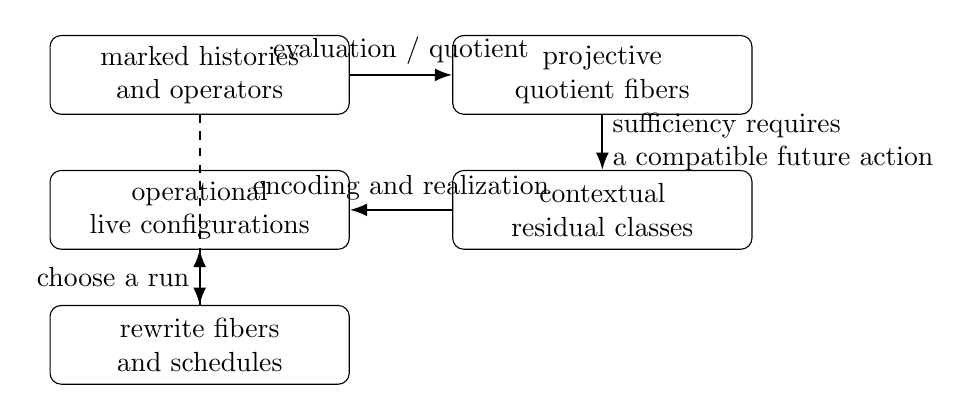
\begin{tikzpicture}[
  node distance=7mm and 13mm,
  box/.style={draw,rounded corners,align=center,minimum width=38mm,minimum height=10mm},
  arr/.style={-{Latex[length=2.2mm]},thick}
]
\node[box] (hist) {marked histories\\and operators};
\node[box,right=of hist] (quot) {projective\\quotient fibers};
\node[box,below=of quot] (res) {contextual\\residual classes};
\node[box,left=of res] (live) {operational\\live configurations};
\node[box,below=of live] (rew) {rewrite fibers\\and schedules};
\draw[arr] (hist) -- node[above]{evaluation / quotient} (quot);
\draw[arr] (quot) -- node[right,align=left]{sufficiency requires\\a compatible future action} (res);
\draw[arr] (res) -- node[above,sloped]{encoding and realization} (live);
\draw[arr] (rew) -- node[left]{choose a run} (live);
\draw[arr,dashed] (hist) -- (rew);
\end{tikzpicture}
\caption{The four layers of Paper~IV.  A projective quotient becomes a
future-sensitive state only after the future action and observation are fixed;
a residual lower bound becomes operational space only after encoding and
machine conventions are fixed.}
\label{fig:intro-four-layers}
\end{figure}

\subsection{Main results}

The paper establishes seven groups of results.

First, we complete the algebraic quotient layer.  A regular bivaluation---an
ordered pair of distinct projective points---is naturally a rank-one
idempotent.  For the ordered-pair stabilizer $H$ and the two point stabilizers
$B_\pm$,
\[
  G/H\cong\Biv_K^{\mathrm{reg}},
  \qquad
  G/B_\pm\cong\PP^1(K).
\]
The principal $H$-torsor $G\to G/H$ is the projective-frame residue over a
condensed projector.  This is algebraic condensation.  It must be distinguished
from convergence of normalized matrix products to a singular rank-one map.

Second, we prove a continuation-side theorem.  Left multiplication by every
future operator descends to $G/H$.  A single right update by $k$ descends
exactly when $k^{-1}Hk\subseteq H$; a reversible right action descends exactly
when $k$ normalizes $H$.  Consequently, the same quotient may be sufficient
for chronological continuation by left composition and insufficient for a
right-composition convention.  The theorem gives an exact meaning to the
statement that forgotten frame data can become visible again.

Third, we define contextual continuation residuals and prove the finite exact
minimal-state theorem.  The quotient by residual equivalence is a canonical
deterministic online state space, in the same structural tradition as the
Nerode equivalence for automata \cite{Nerode1958}.  Any exact implementation
must inject this quotient into its encoded states.  This yields a bit lower
bound and, under an explicit fixed-register snapshot convention, a
capacity--time lower bound.

Fourth, we construct a finite ported-program interface for punctured AES
carriers.  Source- and occurrence-preserving substitution is compatible with
strict partial evaluation on its exact domain.  Network reassociation is an
explicit isomorphism, not equality of literal call receipts.  Compatible
geometric collars and computational interfaces descend together when the
assembled event graph is acyclic.  Feature observation factorization and online
feature update have distinct criteria: contextual refinement and a
right-congruence kernel, respectively.  The attached-program construction does
not supply a faithful realization of its gates by AES motions.

Fifth, we introduce a live-configuration cost vector separating static
description, work, elapsed steps, causal depth, peak workspace, memory--time,
and communication.  We prove that a monotone completed-node set cannot encode
space in models allowing deletion or recomputation.

Sixth, we give a word-fiber and conditional-entropy inequality.  Exponential
raw history growth combined with small evaluation-image growth forces large
operator fibers and large conditional information.  The conclusion is about
an evaluation map.  It is not a time lower bound.  Finite generating sets give
quasi-isometric word metrics, so polynomial versus exponential group growth is
stable under that restricted change of generators, while computational costs
remain model-dependent.

Seventh, exact case studies calibrate the distinctions.  Horner words exhibit
charge condensation; OBDDs exhibit future-residual sensitivity to variable
order; butterflies and NTTs exhibit representation change and static torus
labels; matrix chains and checkpointing exhibit equal semantics with different
work and space; and rewrite potentials exhibit a telescoping obstruction to
nontrivial holonomy.

\subsection{What is not claimed}

No result in this paper asserts any of the implications
\[
  \text{noncommutativity}\Longrightarrow\text{negative curvature},
  \qquad
  \text{negative curvature}\Longrightarrow\text{exponential time},
\]
\[
  \text{exponential word growth}\Longrightarrow\text{NP-hardness},
  \qquad
  \log|\text{fiber}|=\text{workspace}.
\]
The free group already has exponential metric growth while free reduction is
linear in the input-word length.  Conversely, the OBDD example in
Section~\ref{sec:obdd} has an exponential cut-width separation although the
underlying variable restrictions commute.  The appropriate conclusions are
therefore conditional comparison theorems, not a universal scalar complexity
law.

\subsection{Roadmap}

Sections~\ref{sec:history-equality}--\ref{sec:projective-quotients} establish
the history and homogeneous-space layers.  Section~\ref{sec:condensation-continuation}
proves the quotient-continuation results.  Section~\ref{sec:contextual-residuals}
develops residual semantics.  Section~\ref{sec:ported-aes} supplies the finite
ported-program interface, and Section~\ref{sec:operational-resources}
separates semantic state from operational resources.  Sections~\ref{sec:growth-information}
and \ref{sec:rewrite-fibers} treat growth and rewriting.  The four case-study
sections follow.  The final two sections state the claim boundary and the
remaining research programme.  Appendices collect calculations, proof variants,
finite counts, and a theorem-level claim ledger.

\section{Histories, evaluations, and equality levels}\label{sec:history-equality}
% Canonical Paper IV section.
Paper~I defines a marked spinal history as a chronological word of one-hole
arithmetic contexts.  We recall only the structure needed to discuss quotient
fibers and continuation.  Throughout this section $K$ is a field, and all
projective contexts are assumed non-degenerate.

\subsection{Free histories and two semantic categories}

Let $\Sigma_K$ be a selected set of invertible one-hole arithmetic contexts.
It may contain translations, nonzero scalings, sign changes, and inversion.
A free history is a word
\[
  \gamma=s_1s_2\cdots s_n,
  \qquad s_i\in\Sigma_K,
\]
listed in chronological order.  Its induced transformation is
\begin{equation}
  \rho(\gamma)=\rho(s_n)\cdots\rho(s_2)\rho(s_1)
  \in G:=\PGL_2(K).
  \label{eq:chronological-evaluation}
\end{equation}
Thus a newly appended future context acts by left multiplication.  This
chronology convention is essential in Section~\ref{sec:condensation-continuation}.

\begin{definition}[Ordinary and projective evaluation]
For an initial value $x\in K$, ordinary evaluation $\nu_x(\gamma)$ is defined
only when every intermediate arithmetic operation is defined in $K$.
Projective evaluation is the everywhere-defined action of $\rho(\gamma)$ on
$\PP^1(K)$.  We write
\[
  \operatorname{dom}_{\mathrm{ord}}(\gamma)\subseteq K
\]
for the ordinary domain.
\end{definition}

For example, the projective continuation $z\mapsto c/z$ sends $0$ to
$\infty$, while ordinary division by zero is undefined.  The projective target
therefore does not erase the ordinary-domain label.  Later residual definitions
will assign a distinguished observation $\bot$ to an illegal ordinary
continuation.

\begin{definition}[Word-labelled history category]
Let $\cH_K$ have objects $q\in\PP^1(K)$.  A morphism from $q$ to $q'$ is a
pair $(\gamma,q)$ consisting of a literal context word with
$\rho(\gamma)q=q'$.  If $\gamma$ is followed chronologically by $\delta$,
the composite is labelled by the concatenated history $\gamma\star\delta$
and satisfies
\[
  \rho(\gamma\star\delta)=\rho(\delta)\rho(\gamma).
\]
Formal inverses of context symbols give a groupoid completion
$\cH_K^{\mathrm{inv}}$.  Projective evaluation defines a functor
\[
  \rho:\cH_K^{\mathrm{inv}}
  \longrightarrow
  \PP^1(K)\sslash G,
\]
to the action groupoid by forgetting the literal word and retaining its
projective operator.  Distinct word-labelled arrows are not identified merely
because they have the same image in $G$.
\end{definition}

This construction is intentionally modest.  Associativity, commutativity,
distributivity, and program transformations may later be added as rewrite
$2$-cells between word-labelled arrows.  They are not imposed as literal
history equality.

\subsection{The equality tower}

A bounded history $(x,\gamma)$ supports several non-equivalent equality tests.
For compatible histories $\gamma$ and $\delta$, consider:
\begin{align*}
  \gamma&=\delta &&\text{literal history equality},\\
  \rho(\gamma)&=\rho(\delta) &&\text{projective operator equality},\\
  \rho(\gamma)q&=\rho(\delta)q &&\text{equality at a projective state $q$},\\
  \nu_x(\gamma)&=\nu_x(\delta) &&\text{ordinary endpoint equality},\\
  \chi(\gamma)&=\chi(\delta) &&\text{equality of a selected charge shadow}.
\end{align*}
Only the forward implications forced by the selected maps are automatic.
Endpoint equality at one input does not imply operator equality; operator
equality does not imply history equality; and charge equality need not imply
operator equality.  These failures are not pathologies.  They are the fibers
that the present paper studies.

\begin{proposition}[Nested kernel pairs]
Let $X\xrightarrow{f}Y\xrightarrow{g}Z$ be maps.  The kernel pair of $f$ is
contained in the kernel pair of $g\circ f$:
\[
  f(x)=f(x')\quad\Longrightarrow\quad g(f(x))=g(f(x')).
\]
The converse holds exactly when $g$ is injective on $f(X)$.
\end{proposition}
\begin{proof}
The forward implication is functoriality of equality.  If $g$ is injective on
$f(X)$, equality after $g$ implies equality before $g$.  Conversely, if the
converse implication holds for all $x,x'$, then $g$ is injective on the image
of $f$.
\end{proof}

This proposition is the set-theoretic skeleton of the full tower.  Its
computational interpretation requires a future class, developed in
Section~\ref{sec:contextual-residuals}.

\subsection{Group-valued relative defects}

Endpoint subtraction is natural in an affine chart but not projectively
invariant.  The operator group supplies a comparison that survives inversion.

\begin{definition}[Relative projective defect]
For invertible histories $\gamma$ and $\delta$, define
\begin{equation}
  \cK(\gamma,\delta)
  \defeq \rho(\delta)^{-1}\rho(\gamma)\in G.
  \label{eq:relative-projective-defect}
\end{equation}
\end{definition}
It satisfies
\[
  \cK(\gamma,\gamma)=1,
  \qquad
  \cK(\gamma,\delta)^{-1}=\cK(\delta,\gamma),
\]
and the cocycle identity
\begin{equation}
  \cK(\gamma,\eta)
  =\cK(\delta,\eta)\cK(\gamma,\delta).
  \label{eq:defect-cocycle}
\end{equation}

\begin{proposition}[Affine torsion as a coordinate of the relative defect]
Suppose
\[
  \rho(\gamma)(x)=sx+A_\gamma,
  \qquad
  \rho(\delta)(x)=sx+A_\delta,
  \qquad s\ne0.
\]
Then
\[
  \cK(\gamma,\delta)(x)=x+\frac{A_\gamma-A_\delta}{s}.
\]
The ordinary endpoint defect $A_\gamma-A_\delta$ is therefore the translation
coordinate of the projective relative defect, multiplied by the common scale.
\end{proposition}
\begin{proof}
The inverse of $x\mapsto sx+A_\delta$ is
$x\mapsto s^{-1}(x-A_\delta)$.  Composition with the first affine map gives
the formula.
\end{proof}

Once the two operators do not have the same affine linear part, a scalar
endpoint difference depends on the initial value.  Once inversion is admitted,
it may also cross poles.  The group-valued defect remains defined at the
operator level, while its endpoint observation still requires domain data.

\subsection{Relations, neutral histories, and fibers}

\begin{definition}[Operator relation and neutrality]
An ordered pair $(\gamma,\delta)$ is an operator relation when
$\rho(\gamma)=\rho(\delta)$.  A history $\gamma$ is operator-neutral when
$\rho(\gamma)=1$.  It is charge-neutral relative to a charge map $\chi$ when
$\chi(\gamma)$ equals the charge of the empty history.
\end{definition}

Operator-neutral histories form the kernel of $\rho$ only when the history
language has been given a compatible group structure.  In the free monoid they
form a submonoid preimage of the identity; in the formal groupoid they form
isotropy arrows above the relevant object.  Charge-neutral and
operator-neutral histories need not coincide.

\begin{example}[Four elementary separations]
The following examples use affine maps and are proved by direct composition.
\begin{enumerate}
  \item $x\mapsto x+1$ and $x\mapsto2x$ agree at $x=1$ but are different
  operators.
  \item The words ``add $1$, then add $2$'' and ``add $2$, then add $1$'' are
  distinct histories inducing the same map $x\mapsto x+3$.
  \item ``add $p$, then scale by $e^q$'' and the opposite order have the same
  ACS endpoint but differ by translation $p(e^q-1)$.
  \item ``add $p$, then add $-p$'' is a nonempty operator-neutral history.
\end{enumerate}
\end{example}

The operator fiber $\rho^{-1}(g)$ and the endpoint fiber
$\{\gamma:\nu_x(\gamma)=y\}$ are therefore distinct objects.  The first is
independent of $x$; the second need not be.  Paper~IV uses ``history fiber''
only after naming the map whose fiber is intended.

\subsection{Chronological end versus operand slot}

The side on which a future operator is multiplied is not the operand-slot
chirality of an arithmetic context.  Operand-slot chirality records whether
the evolving value occupies the first or second input of one binary operation.
Chronological side records whether a new operator is composed before or after
an existing product.  In the convention \eqref{eq:chronological-evaluation}, a
future context acts on the left regardless of its operand slot.  A theorem
relating slot mirror, matrix transpose, inverse, or right continuation would
require additional structure and is not assumed here.

\section{Bivaluations and the projective quotient tower}\label{sec:projective-quotients}
% Canonical Paper IV section.
The projective operator in Section~\ref{sec:history-equality} is already a
condensation of a marked history.  We now introduce a second, algebraic
condensation: an operator is replaced by the image--kernel pair of a rank-one
projector.  No topology, norm, probability, or limiting dynamics is used in
this section.

\subsection{Points, copoints, and regular bivaluations}

Let $V=K^2$ and let $V^\vee$ be its algebraic dual.  A nonzero vector $v$
defines a point $[v]\in\PP(V)$, while a nonzero covector $\varphi$ defines the
projective line $\PP(\ker\varphi)\in\PP(V)$.  The pair is transverse when
$\varphi(v)\ne0$.

\begin{definition}[Regular bivaluation]
A regular bivaluation over $K$ is an ordered pair
\[
  (q^+,q^-)\in\PP^1(K)\times\PP^1(K),
  \qquad q^+\ne q^-.
\]
The first member is called the image direction and the second the kernel
direction.  We write
\[
  \Biv_K^{\mathrm{reg}}
  \defeq \PP^1(K)\times\PP^1(K)\setminus\Delta.
\]
\end{definition}

The order matters.  Interchanging image and kernel replaces a projector by its
complement.

\begin{theorem}[Bivaluation--projector correspondence]
\label{thm:bivaluation-projector}
There is a natural bijection
\[
  \Biv_K^{\mathrm{reg}}
  \longleftrightarrow
  \{\Pi\in\End(V):\Pi^2=\Pi,\ \rank\Pi=1\}.
\]
If $q^+=[v]$, $q^-=\PP(\ker\varphi)$, and $\varphi(v)\ne0$, the
corresponding projector is
\begin{equation}
  \Pi_{v,\varphi}=\frac{v\otimes\varphi}{\varphi(v)}.
  \label{eq:rank-one-projector}
\end{equation}
\end{theorem}

\begin{proof}
For transverse lines $L^+$ and $L^-$ one has $V=L^+\oplus L^-$.  There is a
unique linear projection onto $L^+$ along $L^-$.  Formula
\eqref{eq:rank-one-projector} gives it and is unchanged if $v$ or $\varphi$
is rescaled.  Conversely, an idempotent splits
$V=\im\Pi\oplus\ker\Pi$.  Rank one makes both summands distinct projective
lines.  The two constructions are inverse.
\end{proof}

In the affine chart
\[
  v_a=\begin{pmatrix}-a\\1\end{pmatrix},
  \qquad
  \varphi_b=\begin{pmatrix}-b&1\end{pmatrix},
\]
one has $\varphi_b(v_a)=1+ab$ and hence
\begin{equation}
  \Pi_{a,b}
  =\frac{1}{1+ab}
    \begin{pmatrix}ab&-a\\-b&1\end{pmatrix}.
  \label{eq:local-projector}
\end{equation}
The divisor $1+ab=0$ is a genuine incidence failure of the transverse
splitting.  It must not be confused with the pole of one particular coordinate
chart.

\subsection{The homogeneous-space tower}

Fix a reference ordered pair $(q_0^+,q_0^-)$ and set
\[
  G=\PGL_2(K),
  \qquad
  H=\Stab_G(q_0^+,q_0^-),
\]
\[
  B_+=\Stab_G(q_0^+),
  \qquad
  B_-=\Stab_G(q_0^-).
\]
Then $H=B_+\cap B_-$.  We use right cosets in $G/H$ and $G/B_\pm$.

\begin{theorem}[Projective quotient tower]
\label{thm:projective-quotient-tower}
There are natural identifications
\[
  G/H\cong\Biv_K^{\mathrm{reg}},
  \qquad
  G/B_+\cong\PP^1(K),
  \qquad
  G/B_-\cong\PP^1(K).
\]
Under these identifications, the maps induced by
$H\subseteq B_\pm$ forget respectively the kernel or image member of the
ordered pair.
\end{theorem}

\begin{proof}
The group $G$ acts transitively on ordered pairs of distinct projective points.
The stabilizer of the reference pair is exactly $H$, so orbit--stabilizer gives
$G/H$.  The same argument for a single projective point gives the two Borel
quotients.  The descriptions of the forgetful maps follow from the subgroup
inclusions.
\end{proof}

Combining this result with projective evaluation gives the central algebraic
tower
\begin{equation}
\boxed{
  \Hist_K
  \xrightarrow{\ \rho\ }
  G
  \xrightarrow{\ \pi_H\ }
  G/H\cong\Biv_K^{\mathrm{reg}}
  \longrightarrow
  G/B_\pm\cong\PP^1(K).
}
\label{eq:paper4-main-tower}
\end{equation}
The first fiber consists of literal histories inducing one operator.  The
second consists of projective frames over one image--kernel result.  These are
different kinds of forgotten data.

\subsection{A third point restores the projective frame}

\begin{definition}[Framed bivaluation]
A framed regular bivaluation is a pairwise distinct ordered triple
$(q^+,q^-,q^\infty)$ of points of $\PP^1(K)$.  The first two determine the
rank-one projector; the third selects a projective frame above it.
\end{definition}

\begin{theorem}[Frame torsor]
\label{thm:frame-torsor}
After a reference triple has been chosen, the set of framed regular
bivaluations is a $G$-torsor.  The projection
\[
  (q^+,q^-,q^\infty)\longmapsto(q^+,q^-)
\]
has fibers on which $H$ acts freely and transitively.  Equivalently,
$G\to G/H$ is an $H$-torsor.
\end{theorem}

\begin{proof}
A projective transformation is uniquely determined by its values on three
distinct projective points.  Hence $G$ acts simply transitively on ordered
projective frames.  Holding the first two points fixed leaves exactly their
stabilizer $H$, which acts simply transitively on the allowed third points.
\end{proof}

For a Lie group this torsor may be equipped with a connection, but no such
connection is canonical over an arbitrary field.  A coordinate in $H$ also
requires a reference lift or local section.

\begin{proposition}[Stabilizer-valued operator residue]
\label{prop:stabilizer-residue}
Let $\Pi_0$ be the projector of the reference bivaluation and define
$\pi_H(g)=g\Pi_0g^{-1}$.  Then
\[
  \pi_H(g_1)=\pi_H(g_2)
  \quad\Longleftrightarrow\quad
  g_2^{-1}g_1\in H.
\]
Thus two operator-level processes with the same condensed projector differ by
an $H$-valued frame residue.
\end{proposition}

\begin{proof}
Equality of the two conjugated projectors is equivalent to
\[
  (g_2^{-1}g_1)\Pi_0(g_2^{-1}g_1)^{-1}=\Pi_0.
\]
The stabilizer of a rank-one projector is precisely the stabilizer of its
ordered image and kernel lines, namely $H$.
\end{proof}

A static idempotent already splits $V=\im\Pi\oplus\ker\Pi$.  It therefore does
not carry a nontrivial linear extension class by itself.  Process information
discarded by $G\to G/H$ belongs instead to a lift, a connection and its
holonomy, or some additional decoration of the history.

\subsection{Finite-field calibration}

\begin{proposition}[Exact finite-field fiber counts]
\label{prop:finite-field-counts}
For $K=\F_q$,
\[
  |\PP^1(\F_q)|=q+1,
  \qquad
  |\Biv_{\F_q}^{\mathrm{reg}}|=q(q+1),
\]
\[
  |\PGL_2(\F_q)|=q(q^2-1),
  \qquad
  |H|=q-1.
\]
Consequently every fiber of
$\PGL_2(\F_q)\to\Biv_{\F_q}^{\mathrm{reg}}$ has $q-1$ elements.
\end{proposition}

\begin{proof}
There are $q+1$ projective points and then $q$ choices for a distinct second
point.  Moreover
$|\GL_2(\F_q)|=(q^2-1)(q^2-q)$; quotienting by the $q-1$ nonzero scalar
matrices gives $q(q^2-1)$.  The stabilizer of $(0,\infty)$ consists of
$z\mapsto az$ with $a\in\F_q^\times$, and hence has order $q-1$.
\end{proof}

\begin{example}[The field $\F_7$]
\label{ex:f7-counts}
One obtains
\[
  |G|=336,
  \qquad |G/H|=56,
  \qquad |H|=6.
\]
The 336 ordered projective frames condense to 56 ordered image--kernel pairs,
with six frame lifts above each pair.
\end{example}

\begin{corollary}[Uniform finite-frame information]
\label{cor:finite-frame-entropy}
Let $G=\PGL_2(\F_q)$ be uniformly distributed and let $Q=gH$.  Then
\[
  H(g\mid Q)=\log_2(q-1).
\]
This is the exact conditional information in the uniformly distributed frame
coordinate above a bivaluation.
\end{corollary}

\begin{proof}
Every quotient fiber has $q-1$ elements and the conditional distribution on
that fiber is uniform.
\end{proof}

The corollary is an algebraic information statement.  Whether these bits are
needed by an online computation depends on the continuation experiment of the
next section.

\subsection{Algebraic and dynamical condensation}

\begin{definition}[Algebraic condensation]
Algebraic condensation is passage to an idempotent or quotient state, such as
$g\mapsto gH$ or $g\mapsto g\Pi_0g^{-1}$.  It requires no limiting sequence.
\end{definition}

\begin{definition}[Dynamical condensation]
Dynamical condensation is convergence, after a declared normalization, of a
sequence of linear lifts to a singular rank-one operator, for example
\[
  \frac{\widetilde g_n\cdots\widetilde g_1}{r_n}
  \longrightarrow \Pi
  \quad\text{in }\End(V).
\]
It requires a topology or valuation, a choice of lifts, and a normalization.
\end{definition}

\begin{proposition}[No automatic dynamical condensation over a finite field]
In the discrete topology on $\PGL_2(\F_q)$, every sequence of powers is
periodic and convergence occurs only when the sequence is eventually constant.
Thus the existence of rank-one idempotents over $\F_q$ does not imply a
nontrivial attracting limit in $G$.
\end{proposition}

The distinction will remain active throughout the paper.  The quotient
$G/H$ is an exact algebraic state space; whether it is sufficient for future
computation is a separate question.

\section{Condensation and future continuation}\label{sec:condensation-continuation}
% Canonical Paper IV section.
A quotient forgets distinctions by definition.  It becomes a computationally
meaningful state only after a future action and an observation have been
specified.  This section gives the exact group-theoretic test for the
projective quotient $G/H$.

\subsection{Equivariant quotients and future sufficiency}

Let a monoid $M$ act on a set $X$ from the left, let $q:X\to Q$ be a
surjection, and suppose an action of $M$ on $Q$ satisfies
\[
  q(mx)=m q(x).
\]
Let $o:Q\to Y$ be an observation.  For $x,x'\in X$, define
\[
  x\equiv_{M,o}x'
  \quad\Longleftrightarrow\quad
  o(mq(x))=o(mq(x'))\quad\text{for every }m\in M.
\]

\begin{theorem}[Equivariant quotient as a residual state]
\label{thm:equivariant-quotient-residual}
If $q(x)=q(x')$, then $x\equiv_{M,o}x'$.  If the identity belongs to $M$ and
$o$ is injective, then the converse also holds.  Under those hypotheses the
future-residual quotient of $X$ is exactly $Q$.
\end{theorem}

\begin{proof}
Equivariance gives $q(mx)=mq(x)=mq(x')=q(mx')$, and applying $o$ proves the
first statement.  For the converse, test the identity continuation.  Then
$o(q(x))=o(q(x'))$, and injectivity of $o$ gives $q(x)=q(x')$.
\end{proof}

The theorem does not say that every quotient is sufficient.  It says that
sufficiency follows from a declared descended action; minimality additionally
uses an observation that can distinguish quotient states.

\subsection{Left continuation on the bivaluation quotient}

For the chronology convention of Equation~\eqref{eq:chronological-evaluation},
a future operator $k$ acts on the current operator $g$ by left multiplication:
$g\mapsto kg$.  The right-coset quotient therefore has the canonical action
\[
  k\cdot(gH)=(kg)H.
\]

\begin{corollary}[Exact left-continuation state]
\label{cor:left-continuation-exact}
Let all elements of $G$ be allowed as left futures, include the identity
future, and observe the resulting point of $G/H$ through an injective map.
Then two operators have the same future behavior exactly when they lie in the
same right coset:
\[
  g\equiv g'\quad\Longleftrightarrow\quad gH=g'H.
\]
Thus $G/H$ is the canonical minimal exact state space for this continuation
experiment.
\end{corollary}

In particular, the $H$-coordinate discarded by projective condensation is
invisible to every left continuation whose observation factors through the
same quotient.

\subsection{Right continuation and the normalizer boundary}

Opposite chronology replaces $g$ by $gk$.  Unlike left multiplication, this
does not automatically act on right cosets.

\begin{theorem}[Descent of one right update]
\label{thm:right-update-descent}
For a fixed $k\in G$, the formula
\[
  R_k(gH)=gkH
\]
defines a well-defined map $G/H\to G/H$ if and only if
\begin{equation}
  k^{-1}Hk\subseteq H.
  \label{eq:right-descent-inclusion}
\end{equation}
It is a bijection with inverse induced by $k^{-1}$ if and only if
$k\in N_G(H)$.
\end{theorem}

\begin{proof}
If $gH=ghH$ with $h\in H$, well-definedness requires
$ghkH=gkH$.  Cancelling $gk$ on the left gives
$k^{-1}hk\in H$ for every $h\in H$, which is
\eqref{eq:right-descent-inclusion}.  The same argument for $k^{-1}$ gives the
reverse inclusion.  Both hold exactly when $k^{-1}Hk=H$, equivalently
$k\in N_G(H)$.
\end{proof}

\begin{corollary}[Reversible right continuation]
\label{cor:right-group-normalizer}
A subgroup $L\le G$ acts on $G/H$ by right multiplication if and only if
$L\subseteq N_G(H)$.
\end{corollary}

For an infinite group, the inclusion in
\eqref{eq:right-descent-inclusion} may be strict, so the single-update and
reversible statements must not be conflated.  For finite $H$, equal
cardinality turns the inclusion into equality.

\begin{corollary}[Chronology-dependent visibility]
Suppose $h\in H$ is discarded by $g\mapsto gH$.  Under left continuation one
always has $kghH=k gH$, so $h$ remains invisible.  Under a right continuation
$k$ for which $k^{-1}hk\notin H$, the two representatives $g$ and $gh$ no
longer determine the same quotient state after continuation.  The discarded
frame direction has become observable.
\end{corollary}

This is the first rigorous bridge between projective process residue and a
future-sensitive residual.  The bridge is not the cardinality of $H$ alone;
it is the interaction between $H$ and the declared continuation side.

\subsection{The split-torus normalizer in rank one}

Take the reference pair $(0,\infty)$.  Then
\[
  H=\{z\mapsto az:a\in K^\times\}.
\]
Let $J(z)=1/z$; the sign is irrelevant projectively.

\begin{proposition}[Normalizer of the ordered-pair stabilizer]
\label{prop:split-torus-normalizer}
If $|K|>2$, then
\[
  N_G(H)=H\sqcup JH.
\]
Equivalently, a projective map normalizes $H$ exactly when it preserves the
unordered set $\{0,\infty\}$; it either fixes the two points or interchanges
them.
\end{proposition}

\begin{proof}
Because $|K|>2$, choose $a\ne1$.  The map $z\mapsto az$ has fixed set exactly
$\{0,\infty\}$.  Hence the common fixed set of $H$ is $\{0,\infty\}$.  A
normalizer sends this common fixed set to itself.  If it fixes both points it
lies in $H$; if it swaps them, composition with $J$ fixes both and lies in
$H$.  Conversely, $H$ normalizes itself and $J(z)=1/z$ conjugates
$z\mapsto az$ to $z\mapsto a^{-1}z$.
\end{proof}

Thus most right projective futures do not descend to the bivaluation quotient.
Remembering only the rank-one projector is sufficient for the left chronology,
but generally insufficient for arbitrary two-sided process composition.

\subsection{Sufficient, exact, and minimal condensations}

\begin{definition}[Future-sufficient condensation]
For a past space $P$, a continuation class $M$, and an observation $\Obs$, a
map $q:P\to Q$ is future-sufficient if there exist descended transitions on
$Q$ and an output map $o:Q\to Y$ such that every observation after every
continuation can be computed from $q(p)$.
\end{definition}

\begin{definition}[Exact and minimal condensation]
A future-sufficient condensation is exact when
$q(p)=q(p')$ precisely for pasts indistinguishable by all allowed futures.  It
is minimal when every other exact deterministic state representation maps
surjectively onto it.
\end{definition}

Theorem~\ref{thm:equivariant-quotient-residual} proves exactness for the
projective left-action experiment.  Section~\ref{sec:contextual-residuals}
gives the general residual construction and proves minimality without assuming
a group quotient.

\subsection{An exact-transport obstruction}

A tempting way to label a path of states is to choose frames $h_t\in G$ and
put
\[
  r_t=h_t h_{t-1}^{-1}.
\]
This transport contains no independent edge information.

\begin{proposition}[Exact edge labels telescope]
\label{prop:exact-transport-telescope}
For $s<t$,
\[
  r_t r_{t-1}\cdots r_{s+1}=h_t h_s^{-1}.
\]
Every closed lifted path therefore has trivial product.
\end{proposition}

\begin{proof}
All intermediate factors cancel pairwise.
\end{proof}

A nontrivial projective process holonomy consequently requires more than an
endpoint potential.  Possible additional data include an independent
stabilizer-valued factor in each edge, a connection on $G\to G/H$, a
multivalued frame, or rewrite $2$-cells.  None is supplied automatically by the
static quotient.

% ======================================================================
% Insert into Paper IV, Section 4, after Subsection 4.6
% (Resolves Open Problem 14.1 in the main flow)
% ======================================================================

\subsection{Non-exact projective transport and cross-ratio holonomy}
\label{subsec:non-exact-projective-transport}

Proposition~\ref{prop:telescoping} shows that edge labels defined solely as ratios
$r_t = h_t h_{t-1}^{-1}$ of vertex frame lifts telescope along every closed path.
To obtain a gauge-equivariant comparison on the frame torsor $G\to G/H$ that reduces
to affine translation torsion on the Borel sector $B_\infty$ while retaining a
nontrivial closed-loop invariant when the kernel point moves, the edge transport
must couple the image step to the preceding kernel covector. The rank-one idempotent
realization of Theorem~\ref{thm:bivaluation-projector} supplies this coupling
canonically without auxiliary metric data.

Let $K$ be a field. Recall from Section~3.1 that in the standard affine chart on
$Biv_K^{\mathrm{reg}}$, a transverse ordered pair $(q^+,q^-)$ with representatives
$v_a = \binom{-a}{1}$ and $\varphi_b = (-b\;\;1)$ satisfies $\varphi_b(v_a)=1+ab\neq 0$
and determines the rank-one projector $\Pi_{a,b} = (1+ab)^{-1} v_a\otimes\varphi_b$.

\begin{definition}[Incidence-coupled projective edge transport]
\label{def:projective-edge-transport}
Let $e: q_1\to q_2$ be a directed step between regular bivaluations
$q_i=(a_i,b_i)\in Biv_K^{\mathrm{reg}}$ that is transverse in the sense that
\[
  \varphi_{b_1}(v_{a_2}) = 1 + a_2 b_1 \neq 0.
\]
Choose frame lifts $g_i = \begin{pmatrix} 1 & -a_i \\ -b_i & 1 \end{pmatrix}
\begin{pmatrix} \Phi_i & 0 \\ 0 & 1 \end{pmatrix} \in G$ with fiber coordinates
$\Phi_i\in K^\times \cong H$. Define the \emph{projective torsion transport} of the
lifted step $\tilde{e}: g_1\to g_2$ as the element of the affine semidirect product
$\mathrm{Aff}(1,K) = K^\times \ltimes K$ given by
\begin{equation}\label{eq:projective-torsion-matrix}
  \mathcal{T}(\tilde{e}) :=
  \begin{pmatrix}
    \Lambda(\tilde{e}) & \Delta\hat{\xi}(\tilde{e}) \\[4pt]
    0 & 1
  \end{pmatrix},
\end{equation}
where the multiplicative holonomy factor and source-normalized translation increment are
\begin{equation}\label{eq:projective-torsion-components}
  \Lambda(\tilde{e}) := \frac{\Phi_2}{\Phi_1}\cdot \frac{1 + a_2 b_1}{1 + a_1 b_1} \in K^\times,
  \qquad
  \Delta\hat{\xi}(\tilde{e}) := -\Phi_1^{-1}\,\frac{a_2 - a_1}{1 + a_1 b_1} \in K.
\end{equation}
For a multi-step lifted path $\tilde{\gamma}=(\tilde{e}_1,\dots,\tilde{e}_m)$, its
total transport is the chronological product
$\mathcal{T}(\tilde{\gamma}) := \mathcal{T}(\tilde{e}_m)\cdots\mathcal{T}(\tilde{e}_1)
\in\mathrm{Aff}(1,K)$.
\end{definition}

The factor $\lambda_{\mathrm{base}}(e) := (1+a_2 b_1)/(1+a_1 b_1) =
\varphi_{b_1}(v_{a_2})/\varphi_{b_1}(v_{a_1})$ depends only on the base step
$q_1\to q_2$ in $G/H$. Under a change of frame section $\Phi_i \mapsto c_i \Phi_i$,
the product of $\Lambda(\tilde{e}_k)$ around any closed lifted loop
($\Phi_m=\Phi_0$) is strictly gauge-invariant.

\begin{theorem}[Borel reduction and non-telescoping cross-ratio holonomy]
\label{thm:projective-torsion-solution}
The transport $\mathcal{T}$ of Definition~\ref{def:projective-edge-transport}
has the following properties:
\begin{enumerate}
  \item \emph{(Exact Borel reduction).} On the affine Borel sector
  $B_\infty = \mathrm{Stab}_G(\infty)$, where $b_k\equiv 0$ and $a_k=-\xi_k$ for
  every prefix $g_k(z)=\Phi_k z + \xi_k$, the base correction satisfies
  $\lambda_{\mathrm{base}}(e_k)\equiv 1$, and the total transport along a history
  $\gamma=(s_1,\dots,s_n)$ reduces to
  \[
    \mathcal{T}(\gamma)\big|_{B_\infty}
    = \begin{pmatrix} \Phi_n & \xi_n \\ 0 & 1 \end{pmatrix}.
  \]
  Consequently, for scale-compatible affine histories $\gamma$ and $\delta$, the
  translation component of $\mathcal{T}(\delta)^{-1}\mathcal{T}(\gamma)$ is
  precisely the relative affine defect $\Phi^{-1}(\xi_\gamma - \xi_\delta)$ of
  Paper~0, Section~7.4.

  \item \emph{(Fixed-kernel flatness).} Along any closed lifted loop $\ell$ on which
  the kernel coordinate $b_k\equiv b_0$ remains constant, the multiplicative
  holonomy telescopes to $\Lambda(\ell)=1$.

  \item \emph{(Non-telescoping cross-ratio holonomy).} Consider a closed four-step
  base loop $\square$ in $Biv_K^{\mathrm{reg}}$ alternating image updates and kernel
  updates:
  \[
    (a_1,b_1) \xrightarrow{e_1} (a_2,b_1) \xrightarrow{e_2} (a_2,b_2)
    \xrightarrow{e_3} (a_1,b_2) \xrightarrow{e_4} (a_1,b_1),
  \]
  where all four pairs and intermediate steps are transverse. For any closed frame
  lift ($\Phi_4=\Phi_0$), the multiplicative holonomy around $\square$ is
  gauge-invariant and equals the projective cross-ratio
  \begin{equation}\label{eq:cross-ratio-holonomy}
    \Lambda(\square)
    = \mathrm{tr}\!\left(\Pi_{a_1,b_1}\Pi_{a_1,b_2}\Pi_{a_2,b_2}\Pi_{a_2,b_1}\right)^{-1}
    \text{-normalized}
    = \frac{(1+a_2 b_1)(1+a_1 b_2)}{(1+a_1 b_1)(1+a_2 b_2)}
    = 1 - \frac{(a_2-a_1)(b_2-b_1)}{(1+a_1 b_1)(1+a_2 b_2)}.
  \end{equation}
  In particular, $\Lambda(\square)\neq 1$ if and only if $a_1\neq a_2$ and $b_1\neq b_2$.
\end{enumerate}
\end{theorem}

\begin{proof}
(1) Setting $b_k=0$ and $a_k=-\xi_k$ in~\eqref{eq:projective-torsion-components}
gives $\Lambda(\tilde{e}_k)=\Phi_k/\Phi_{k-1}$ and
$\Delta\hat{\xi}(\tilde{e}_k)=\Phi_{k-1}^{-1}(\xi_k-\xi_{k-1})$. Multiplying the
matrices~\eqref{eq:projective-torsion-matrix} chronologically from $k=1$ to $n$
yields upper-left entry $\Phi_n/\Phi_0=\Phi_n$ and upper-right entry
$\Phi_n \sum_{k=1}^n \Phi_k^{-1}(\xi_k-\xi_{k-1}) = \xi_n$, matching the affine
cocycle law of Paper~0, Proposition~7.1.

(2) If $b_k=b_0$ for all $k$, then $\lambda_{\mathrm{base}}(e_k)=(1+a_k b_0)/(1+a_{k-1}b_0)$,
whose product over a closed loop $a_m=a_0$ cancels pairwise, while $\prod (\Phi_k/\Phi_{k-1})=1$.

(3) Along the four edges of $\square$, the telescoping factors $\Phi_k/\Phi_{k-1}$
cancel. On $e_2: (a_2,b_1)\to(a_2,b_2)$ and $e_4: (a_1,b_2)\to(a_1,b_1)$, the image
coordinate is constant, so $\lambda_{\mathrm{base}}(e_2)=\lambda_{\mathrm{base}}(e_4)=1$.
On $e_1$ and $e_3$, one has $\lambda_{\mathrm{base}}(e_1)=(1+a_2 b_1)/(1+a_1 b_1)$
and $\lambda_{\mathrm{base}}(e_3)=(1+a_1 b_2)/(1+a_2 b_2)$. Their product is
\eqref{eq:cross-ratio-holonomy}. Subtracting numerator and denominator gives
$(1+a_1 b_1)(1+a_2 b_2) - (1+a_2 b_1)(1+a_1 b_2) = (a_2-a_1)(b_2-b_1)$, which is
nonzero precisely when both coordinates move. Direct multiplication of the rank-one
projectors~\eqref{eq:chart-projector} gives
$\Pi_{a_1,b_1}\Pi_{a_1,b_2}\Pi_{a_2,b_2}\Pi_{a_2,b_1} = \Lambda(\square)^{-1}\Pi_{a_1,b_1}$,
confirming that $\Lambda(\square)$ is a chart-independent invariant of the four
idempotents in $G/H$.
\end{proof}

\begin{remark}[Infinitesimal reductive connection over $\mathbb{R}$ or $\mathbb{C}$]
Over $K=\mathbb{R}$ or $\mathbb{C}$, let $\Pi_0=\begin{pmatrix}0&0\\0&1\end{pmatrix}$
be the reference projector at $(0,\infty)$. The reductive splitting
$\mathfrak{pgl}_2 = \mathfrak{h}\oplus\mathfrak{m}$ defined by the eigenspaces of
$\mathrm{ad}(\Pi_0)$ equips the principal $H$-bundle $G\to G/H$ with the connection
one-form $\omega_H = \Phi^{-1}d\Phi + (1+ab)^{-1}(a\,db - b\,da)$ and horizontal
solder component $\theta_+ = \Phi^{-1}(1+ab)^{-1}da$. The first-order expansion of
$\Lambda(\square)$ in~\eqref{eq:cross-ratio-holonomy} is the para-K\"ahler curvature
two-form $(1+ab)^{-2}da\wedge db$ on $Biv_K^{\mathrm{reg}}$, while $\theta_+|_{b=0}
= -\Phi^{-1}da = e^{-M}d\xi$ recovers the left Maurer-Cartan translation form of
Paper~0, Equation~(58).
\end{remark}

\begin{example}[Exact calibration over $\mathbb{F}_7$]
\label{ex:f7-cross-ratio-holonomy}
In the finite-field calibration $K=\mathbb{F}_7$ of Example~\ref{ex:f7-counts}
($|G|=336$, $|G/H|=56$, $|H|=6$), consider the closed bivaluation loop $\square$
with vertices
\[
  (a_1,b_1)=(0,0), \quad (a_2,b_1)=(1,0), \quad (a_2,b_2)=(1,1), \quad (a_1,b_2)=(0,1).
\]
Here $1+a_i b_j \in \{1,2\}\subset\mathbb{F}_7^\times$, so all four vertices and steps
are transverse. Evaluating~\eqref{eq:cross-ratio-holonomy} in $\mathbb{F}_7^\times$ gives
\[
  \Lambda(\square) \equiv \frac{(1+0)(1+0)}{(1+0)(1+1)} \equiv 2^{-1} \equiv 4 \pmod 7.
\]
Thus $\Lambda(\square)=4\neq 1$ in $H\cong\mathbb{F}_7^\times$, providing an explicit
finite witness of non-telescoping projective holonomy.
\end{example}
\section{Contextual residuals and minimal exact state}\label{sec:contextual-residuals}
% Canonical Paper IV section.
The projective quotient in Section~\ref{sec:condensation-continuation} is one
instance of a more general construction.  A past is relevant only through the
effects it can still have on legal futures.  The definition must therefore
name the interface, the future class, the observation, and the treatment of
partial domains.

\subsection{Typed interfaces and totalized partial action}

Fix a typed interface $C$.  Let $P_C$ be the set of admissible pasts reaching
that interface and let $M_C$ be a monoid of future continuations.  Composition
is written as a right action $p\cdot\eta$ and may initially be partial because
ordinary arithmetic, typing, or resource rules can make a continuation
illegal.  Before totalizing, require a domain-compositional partial action:
$p\cdot(\zeta\eta)$ is defined exactly when $p\cdot\zeta$ and
$(p\cdot\zeta)\cdot\eta$ are defined, and their values then agree.
Execution of the free continuation word monoid has this property.  Quotienting
words by an operation relation requires a separate proof that the relation
preserves both values and ordinary domains; projective cancellation alone does
not supply one.

If the action is partial, introduce an absorbing state $\bot$ and put
\[
  P_C^\bot=P_C\sqcup\{\bot\}.
\]
If the action is already total, use the convention $P_C^\bot=P_C$ and adjoin
nothing.  In the partial case, totalize the action by declaring an illegal
continuation to have value $\bot$ and by setting
$\bot\cdot\eta=\bot$.  Let
\[
  O_C:P_C^\bot\longrightarrow Y_C^\bot
\]
be the current observation, with $O_C(\bot)=\bot$ when the absorbing state
is present and $\bot$ is distinct from every valid observation.  Depending on the problem,
$O_C$ may record an endpoint, a projective state, a Boolean answer, a tensor, a
trace, or a distribution.

\begin{definition}[Contextual continuation equivalence]
\label{def:contextual-equivalence}
For $p,p'\in P_C^\bot$, define
\begin{equation}
  p\equiv_C p'
  \quad\Longleftrightarrow\quad
  O_C(p\cdot\eta)=O_C(p'\cdot\eta)
  \quad\text{for every }\eta\in M_C.
  \label{eq:contextual-equivalence}
\end{equation}
The quotient
\[
  \cR_C=P_C^\bot/{\equiv_C}
\]
is the contextual continuation-residual space at $C$.
\end{definition}

The absorbing outcome is essential for partial arithmetic.  Two pasts are not
identified merely because all common legal continuations agree if one of them
admits a future that the other does not.

\begin{proposition}[Equivalence, refinement, and observation monotonicity]
\label{prop:residual-basic-properties}
The relation $\equiv_C$ is an equivalence relation.  Enlarging the continuation
class can only refine it.  Replacing $O_C$ by a coarser observation
$f\circ O_C$ can only coarsen it.
\end{proposition}

\begin{proof}
Reflexivity, symmetry, and transitivity hold pointwise for every continuation.
A larger family supplies more equality tests.  Applying a function to equal
observations preserves equality and can identify previously distinct values.
\end{proof}

Thus a residual is never absolute.  It is relative to a declared experimental
interface.

\subsection{Residuals form the canonical continuation machine}

\begin{proposition}[Right congruence]
\label{prop:residual-right-congruence}
If $p\equiv_Cp'$, then for every $\zeta\in M_C$,
\[
  p\cdot\zeta\equiv_Cp'\cdot\zeta.
\]
Consequently the formula
\[
  [p]\cdot\zeta=[p\cdot\zeta]
\]
defines a right action of $M_C$ on $\cR_C$.
\end{proposition}

\begin{proof}
For every further continuation $\eta$,
\[
  O_C((p\cdot\zeta)\cdot\eta)
  =O_C(p\cdot(\zeta\eta))
  =O_C(p'\cdot(\zeta\eta))
  =O_C((p'\cdot\zeta)\cdot\eta).
\]
\end{proof}

The identity continuation shows that
\[
  \overline O_C([p])=O_C(p)
\]
is well defined.  Hence $(\cR_C,M_C,\overline O_C)$ is itself an exact
deterministic continuation machine.

\begin{definition}[Exact deterministic online realization]
An exact deterministic online realization of the experiment at $C$ consists
of a state set $S$, a right action of $M_C$ on $S$, an encoding
$e:P_C^\bot\to S$, and an output map $o:S\to Y_C^\bot$ such that
\begin{equation}
  e(p\cdot\eta)=e(p)\cdot\eta,
  \qquad
  o(e(p))=O_C(p).
  \label{eq:exact-machine-equivariance}
\end{equation}
The first identity includes the totalized invalid state when necessary.
\end{definition}

The equivariance requirement prevents a representation from being called an
online state merely because a separate external procedure knows the entire
past and recomputes transitions from it.

\begin{theorem}[Canonical minimal exact state]
\label{thm:minimal-exact-residual}
For every exact deterministic online realization there is a unique surjective
$M_C$-equivariant map
\[
  \phi:e(P_C^\bot)\longrightarrow\cR_C
  \qquad\text{with}\qquad
  \phi(e(p))=[p].
\]
It also preserves outputs.  Therefore $\cR_C$ is the canonical minimal
reachable exact state space, up to isomorphism.
\end{theorem}

\begin{proof}
If $e(p)=e(p')$, then for every $\eta$ equivariance and output correctness give
\[
 O_C(p\cdot\eta)
 =o(e(p)\cdot\eta)
 =o(e(p')\cdot\eta)
 =O_C(p'\cdot\eta).
\]
Hence $p\equiv_Cp'$, so $\phi$ is well defined.  It is surjective by definition
of $\cR_C$.  Equivariance follows from
Proposition~\ref{prop:residual-right-congruence}, and output preservation follows
from the identity continuation.  Uniqueness is forced on every reachable state
$e(p)$.
\end{proof}

This is the finite-state principle behind the classical theory of residual
languages and automata~\cite{Nerode1958}, but the present formulation permits
arbitrary typed observations and partial arithmetic domains.

\subsection{Finite-state information lower bound}

\begin{corollary}[Fixed-width exact-state bound]
\label{cor:residual-bit-bound}
Assume $\cR_C$ is finite.  If an exact reachable state is stored in a fixed
$b$-bit register, then
\begin{equation}
  b\ge \left\lceil\log_2|\cR_C|\right\rceil.
  \label{eq:residual-bit-bound}
\end{equation}
The same conclusion holds for a prefix-free variable-length encoding whose
maximum codeword length is $b$.
\end{corollary}

\begin{proof}
Theorem~\ref{thm:minimal-exact-residual} requires at least $|\cR_C|$ reachable
code states.  A fixed $b$-bit register has at most $2^b$ states.  For a
prefix-free code of maximum length $b$, Kraft's inequality also gives at most
$2^b$ codewords.
\end{proof}

The theorem is a state-selection lower bound.  It does not determine the size
of a transition table, the cost of computing the encoding, the time needed to
apply a continuation, or the materialized size of a structured value.

\begin{corollary}[Fixed-register capacity--time bound]
\label{cor:capacity-time-bound}
Consider declared cuts $C_0,\ldots,C_T$.  Suppose that at cut $C_t$ a complete
exact state for every admissible past must fit in a fixed-width register of
capacity $b_t$ bits, and charge one full register snapshot at each cut.  Then
\begin{equation}
  \sum_{t=0}^{T} b_t
  \ge
  \sum_{t=0}^{T}
  \left\lceil\log_2|\cR_{C_t}|\right\rceil.
  \label{eq:capacity-time-bound}
\end{equation}
If $|\cR_{C_t}|\ge c t^d$ eventually, the right side is
$\Omega(T\log T)$; if $|\cR_{C_t}|\ge c a^t$ with $a>1$, it is
$\Omega(T^2)$.
\end{corollary}

\begin{proof}
Apply Corollary~\ref{cor:residual-bit-bound} at each cut and sum.  The two
asymptotic statements follow from summing $\log t$ and $t$, respectively.
\end{proof}

Equation~\eqref{eq:capacity-time-bound} is deliberately called a
capacity--time bound.  It becomes an actual memory--time bound for a run only
when the operational model charges the complete register as live memory at
each snapshot.  Variable-size structured states, compression, communication,
and recomputation require the model of Section~\ref{sec:operational-resources}.

\subsection{Three projective residual experiments}

The quotient tower supplies three different experiments.

\begin{enumerate}
  \item If pasts are operators $g\in G$, futures act on the left, and the
  observation is the bivaluation $gH$, then
  $\cR\cong G/H$ by Corollary~\ref{cor:left-continuation-exact}.

  \item If the observation remembers only $gq_0^+$ and futures continue to act
  on the left, then the residual is $G/B_+$.  The kernel direction has become
  observationally irrelevant.

  \item If arbitrary reversible futures act on the right, $G/H$ does not
  support the action unless the futures lie in $N_G(H)$.  A full operator lift,
  or another state carrying the missing frame information, is then required.
\end{enumerate}

Thus projective process residue can coincide with a continuation residual, map
to one, or be necessary to refine one.  Which case occurs is a theorem about
the chosen action and observation, not a property of the static fiber alone.

\subsection{Randomized and approximate boundaries}

Definition~\ref{def:contextual-equivalence} uses exact deterministic equality.
A randomized algorithm may permit equal output distributions rather than equal
outputs; an approximate algorithm may identify observations within a metric or
loss tolerance; a statistical model may retain only a sufficient statistic for
a declared distribution family.  Each change alters the residual relation and
its lower bound.  No such approximation theorem is inferred from
Corollary~\ref{cor:residual-bit-bound}; approximate residual geometry remains an
open programme.

\section{Ported AES: substitution, execution, and composition}\label{sec:ported-aes}
% Canonical Paper IV section, adapted from the 2026-10-09 ported-AES candidate.
% Source/provenance and mathematical-status integration are recorded in governance.
The residual theory specifies when a state retains enough information for
future computation.  We now give a finite program interface that can be
attached to a punctured AES without identifying its geometry with its program.
Paper~0 owns the carrier geometry and its compactification
\cite{Yuan2026AEGPaperZero}; Paper~I supplies marked one-hole histories
\cite{Yuan2026AEGFoundations}.  The construction here is a structural proposal
for ported realizations.  Its finite-network and descent results are proved
with the hypotheses stated below.  The program/source distinction follows the
interface discipline of the Adva program--process core
\cite{Yuan2026AdvaProgramProcessCore}.

\subsection{Three kinds of opening}

An essential geometric puncture is a declared end where the given assignment
and metric do not extend as regular AES data.  A computational hole is an
ordered place for program substitution.  A port is an input or output interface
associated with a geometric end or a specified regular interface location.
Their identification requires additional data.

\begin{definition}[Ported AES realization proposal]
\label{def:ported-aes-realization}
Let $E=(M,g,a;\mu,\lambda)$ be an oriented regular AES with a declared
compactified carrier and marked end set $S$, where $|S|=k$.  A ported
realization consists of ordered typed port families $I,O$, an anchoring map
\[
  \pi:I\sqcup O\longrightarrow S\sqcup L,
\]
where $L$ is a declared set of regular interface locations, a finite typed
program decoration, and source, occurrence, boundary, and assembly records.
The map $\pi$ is not assumed injective or surjective.  Ports at a puncture carry
data in its end interface; they are not regular points with a value $a(p)$.
\end{definition}

The three integers $k,|I|,|O|$ are independent.  A three-output experiment
declares $|O|=3$; its internal input frontier may have any finite size.  If all
ports anchor injectively into $S$, then $k\ge |I|+|O|$; equality follows for a
bijection.  Ends without ports and ends carrying several ports are allowed.
The roles of the outputs must be declared.  They are not automatically three
scalar values or Adva's construction/space/time views; the outer interface and
the internal frontier are distinct \cite{Yuan2026AdvaTriadicFrontiers}.

Input binding retains the AES geometry unless a separate parameter family
$(g_\theta,a_\theta)$ is supplied.  Such a family needs a proof of the AES
identity, its admissible parameter domain, and its marked end behavior.
Binding is also distinct from topological capping.

\subsection{Finite programs, sources, and occurrences}

\begin{definition}[Strict finite arithmetic network]
\label{def:strict-finite-network}
An open network $P:A\rightsquigarrow B$ is a finite directed acyclic graph
with ordered typed input and output boundaries and ordered input/output slots
at every gate.  Each wire has one producer and one consumer, counting an
external output as a consumer.  Copy and discard are explicit gates.
Primitive gates denote deterministic partial functions.  Source identities are
immutable; distinct uses have distinct occurrence identities, even if their
sources or values agree.  External boundary positions likewise have occurrence
identities separate from source identities.
\end{definition}

The arithmetic fragment used below has exact rational constants, addition,
subtraction, multiplication, division, explicit copy, and strict discard.
Strict discard requires its input producer to be defined.  Thus
$\operatorname{discard}(1/0)$ remains outside the domain.  A finite acyclic
network cannot exhibit feedback divergence; feedback, side effects, and
unbounded interpretation need separately declared semantics.

Repeated use of a program template first creates separate named instances.
Their event occurrences are fresh; their original sources remain the same.
Administrative wire and event renaming then acts on those instances without
changing source or occurrence identity.  Here a source label names the declared
syntactic origin of a gate or wire occurrence.  The ancestry of a value supplied
after substitution is separately recovered from the connected producer DAG and
binding receipt; binding does not overwrite a body's immutable source labels.
Template reuse is therefore distinct from implicit sharing of one produced wire.

\subsection{Program substitution and its receipts}

Let $P$ have ordered holes $i_1,\ldots,i_m$, and let $q_1,\ldots,q_r$ be
already instantiated producer programs.  A binding $\beta$ matches producer
output occurrences to selected holes, preserving types and positions.  Every
supplied output is used once, and every selected hole is filled once.  Unused
outputs require an explicit discard; multiple uses require an explicit copy.
Holes not selected by a partial binding remain on the open frontier.  Fix the
external order as producer inputs in argument order, followed by the unfilled
body inputs.  Sequential partial filling with open producers can induce a
different order from simultaneous filling; comparison then requires a declared
typed boundary permutation.  The closed-producer example below requires none.

\begin{construction}[Certified simultaneous substitution]
\label{constr:certified-substitution}
Take disjoint administrative copies of the body and producer graphs, identify
the matched boundary wires, and retain all primitive gate occurrences and
sources.  Record the ordered binding, producer regions, body region, and call
nesting in a graft receipt.  The resulting network is
\[
  \Subst_\beta(P;\boldsymbol q).
\]
Accept it only when the resulting global graph is acyclic and its boundary
inventory is complete.  A numerical input is admitted by an explicit constant
producer with its source record, rather than by erasing the producing process.
\end{construction}

For ordinary one-way substitution, producers depend only on their external
inputs and the body depends on their outputs, so acyclicity follows.  General
seam assembly has no such guarantee: two locally acyclic pieces can form a
cycle after cross-wiring.  The notation $\Subst$ is reserved for program
substitution; $\Fill$ in Section~\ref{sec:rewrite-fibers} continues to denote
rewrite filling area.

\begin{proposition}[Type and identity preservation]
\label{prop:ported-substitution-preservation}
A legal substitution preserves boundary typing, primitive gate slot order,
source identities, and instantiated gate occurrences.  Distinct occurrences
are not identified by equality of numerical value.
\end{proposition}
\begin{proof}
The disjoint copies separate administrative names.  The binding changes only
which wire supplies a selected body input; it creates no primitive gate and
deletes none.  Its injectivity on producer output occurrences and selected
holes preserves the single-consumer rule.  Source and occurrence records are
transported by the stated renaming map.  The remaining boundaries retain their
declared order.  All other identifications are excluded by construction.
\end{proof}

\subsection{Substitution and partial evaluation}

Write $D_P$ for the strict numerical domain of $P$: inputs for which every
primitive gate required by the network is defined, including producers
eventually consumed by discard.  Primitive numerical functions are pure; no
primitive observes the scheduler.  The numerical result is therefore
independent of the chosen topological schedule.  An operational trace, its
first observed failure, and its costs can still depend on that schedule.

\begin{theorem}[Substitution--evaluation compatibility]
\label{thm:ported-substitution-evaluation}
Let $Q:X\rightsquigarrow A$ and $P:A\times Z\rightsquigarrow B$ be
compatible strict finite networks.  For the binding consuming all outputs of
$Q$, their composite has domain
\begin{equation}
  D_{P\circ Q}
  =\{(x,z):x\in D_Q,\ (\operatorname{Eval}(Q)(x),z)\in D_P\}.
  \label{eq:ported-composite-domain}
\end{equation}
On exactly this domain,
\begin{equation}
  \operatorname{Eval}(P\circ Q)(x,z)
  =\operatorname{Eval}(P)(\operatorname{Eval}(Q)(x),z).
  \label{eq:ported-composite-evaluation}
\end{equation}
The same statement applies to finitely many disjoint producers and partial
filling, retaining the unfilled boundary.
\end{theorem}
\begin{proof}
Use a topological order with producer gates before body gates.  A producer gate
has precisely the same ordered inputs, primitive partial function, and domain
predicate as in $Q$.  Induction gives the same values on its output wires
whenever the producer is defined.  The bound body inputs are therefore exactly
$\operatorname{Eval}(Q)(x)$.  A second topological induction through the body
gives its original gate values and domain predicates.  Every gate of the
composite is consequently defined if and only if both conditions in
Equation~\eqref{eq:ported-composite-domain} hold.  This proves both equations.
Purity permits a different topological order without changing the successful
result or whether all gates are defined; it does not identify ordered traces.
\end{proof}

\begin{corollary}[Three equality levels for composition]
\label{cor:ported-composition-equalities}
Compatible composition has the following laws.
\begin{enumerate}
  \item Partial numerical functions satisfy identity and associativity
  strictly, including equality of their domains.
  \item Operation networks satisfy these laws up to an explicit isomorphism
  of administrative names and contraction of administrative port segments.
  The isomorphism preserves instantiated occurrences, sources, types, slot
  orders, and ordered external boundaries.  Identity networks use the same
  source and occurrence contract as the interface object they preserve.
  \item Literal receipts for different calls or parenthesizations remain
  distinct.  Their final operation networks are related by the preceding
  transport certificate, not by deleting the call history.
\end{enumerate}
\end{corollary}
\begin{proof}
Equation~\eqref{eq:ported-composite-domain} applied twice gives the same three
domain conditions for either parenthesization;
Equation~\eqref{eq:ported-composite-evaluation} then gives the same result.
At graph level, both constructions contain the same instantiated primitive
gates and the same final boundary identifications.  Map each renamed gate and
wire to its counterpart and contract only administrative segments.  This
supplies the stated isomorphism.  A receipt records the actual calls and their
nesting, which these operations do not make equal.
\end{proof}

\subsection{Joint geometric and computational descent}

\begin{proposition}[Collar and interface descent]
\label{prop:ported-collar-descent}
Suppose finitely many oriented regular AES pieces have the same signed
parameters $(\mu,\lambda)$, and orientation-compatible open collar maps
$\phi_{vw}$ produce a Hausdorff smooth surface.  Require inverse and cocycle
conditions and, on every overlap,
\[
  a_v=a_w\circ\phi_{vw},\qquad g_v=\phi_{vw}^{*}g_w.
\]
Require computational seam records to agree on ordered ports, types, sources,
occurrences, gate parameters, and boundary wire identities, with a complete
assembly record for nonlocal relations.  Require the assembled global program
to be a finite DAG.  Require marked end identities and the anchoring map $\pi$
to be compatible with all identifications.

Then the AES data and the computational network descend together.  The
canonical arithmetic frames transform by the collar Jacobians.  The assembled
program obeys Theorem~\ref{thm:ported-substitution-evaluation} for every
compatible causal composition across its interfaces.
\end{proposition}
\begin{proof}
Overlap equality descends the smooth function and positive definite metric.
The identity $|\mathrm da|_g^2=\mu^2+\lambda^2a^2$ is tensorial and holds in
every local chart, hence globally.  Compatible orientation and equal signed
parameters give the same canonical frame formula in each chart, so those
frames also descend.  The seam inventory identifies precisely the specified
wire occurrences without merging sources or introducing implicit copies.
Compatible end markings and anchoring maps descend the attachment of ports to
the carrier.  Global acyclicity yields a topological execution order.  The
numerical composition result follows from the finite-network theorem.
\end{proof}

\begin{warning}[The motion bridge remains additional]
\label{warn:ported-motion-bridge}
Proposition~\ref{prop:ported-collar-descent} does not prove that a gate of the
attached network is an AES motion.  Such a realization requires primitive
partial state transformations $\Phi_\omega$, exact domains, parameter/source
transport, and overlap equations
\[
  T_{vw}\circ\Phi^v_\omega=\Phi^w_\omega\circ T_{vw}
\]
on their stated domains.  Binary gates, explicit copy/discard, and negative
scalings cannot be inferred from the single-value positive affine model.
Full-state tangential residuals must also be retained: an identity arithmetic
word on assignment values need not be the identity on AES states.  Attaching a
program to a surface does not establish a faithful arithmetic-motion
realization.
\end{warning}

For an already given genus-zero $k$-end carrier, $k\ge3$, a pants
decomposition has $k-2$ three-end pieces and $k-3$ internal seams.  Restrict
all data and retain the overlap and assembly records.  Joint descent then
recovers the original ported object.  A second decomposition gives another
atlas of that same object.  Each three-end piece may have punctures and seam
boundaries; it is not thereby a complete three-cusp AES.  Conformal point
compactification additionally requires punctured-disc ends.  These geometric
constructions and distinctions belong to Paper~0
\cite{Yuan2026AEGPaperZero}.

Local block frontiers can alternate across a seam.  Even when the global event
graph is acyclic, the coarse graph whose vertices are whole geometric pieces
may contain a cycle.  One then cannot execute each whole piece just once in a
block order; execution uses the global causal event order and the exposed
seam frontier.

\subsection{Features and future computation}

Fix the experiment $(P_C,M_C,O_C)$ of
Section~\ref{sec:contextual-residuals}, with its declared treatment of illegal
arithmetic.  Use a domain-compositional partial action, or the free
continuation word monoid, before totalization; do not import unproved operation
relations.  Divergence is not identified with a type error or division by zero.
Here $\cdot$ is a declared total right action on $P_C^\bot$, for example
execution of continuation words with an absorbing illegal state and a distinct
invalid observation.  Contextual equivalence means
\[
  p\equiv_Cp'
  \quad\Longleftrightarrow\quad
  O_C(p\cdot\eta)=O_C(p'\cdot\eta)
  \quad\text{for every }\eta\in M_C.
\]
A right congruence is an equivalence relation preserved by every continuation.

Let $\chi_C:P_C^\bot\to Z_C$ be a proposed feature.  It may retain a scalar,
operator, marking, source/occurrence package, or residual.  The kind of feature
and its observation policy are part of the interface.

\begin{theorem}[Feature observation descent]
\label{thm:feature-observation-descent}
The following conditions are equivalent.
\begin{enumerate}
  \item For every declared continuation $\eta$, there is a function $o_\eta$
  on the reachable feature image satisfying
  \[
    o_\eta(\chi_C(p))=O_C(p\cdot\eta).
  \]
  \item $\ker\chi_C$ is contained in contextual continuation equivalence:
  \[
    \chi_C(p)=\chi_C(p')\quad\Longrightarrow\quad p\equiv_Cp'.
  \]
\end{enumerate}
Legal-domain differences are included through the declared invalid outcome.
\end{theorem}
\begin{proof}
The first condition makes all future observations equal on each feature fiber,
which is exactly the second condition.  Conversely, define $o_\eta$ using any
representative of a feature fiber; the second condition makes the choice
immaterial.  This is existence of observation factorization, not an assertion
that the factors can be computed efficiently or at all.
\end{proof}

\begin{proposition}[Online feature update]
\label{prop:feature-online-update}
Feature transitions $u_\eta$ satisfying
\[
  u_\eta(\chi_C(p))=\chi_C(p\cdot\eta)
\]
exist on the reachable image if and only if $\ker\chi_C$ is a right
congruence.  Together with factorization of $O_C$, they give an exact feature
continuation machine.  An executable implementation still requires effective
transition and observation maps.
\end{proposition}
\begin{proof}
Necessity follows by applying $u_\eta$ to equal feature values.  For sufficiency,
define $u_\eta$ by any representative.  Right congruence makes it well defined,
and the action laws descend from the given action.  Output factorization
supplies the current observation.
\end{proof}

\begin{example}[Observation sufficiency without online update]
\label{ex:feature-not-online}
Take states $0,1,2$, constant observation zero, and the idempotent update
$f(0)=0$, $f(1)=2$, $f(2)=2$.  Every state is contextually equivalent for the
monoid $\{\id,f\}$.  Let $\chi(0)=\chi(1)=0$, $\chi(2)=1$.
Feature observation descent holds, but $\chi(f(0))\ne\chi(f(1))$, so no
feature update can be defined on input feature zero.  A future-sufficient
observation and a closed online state are different requirements.
\end{example}

Actual opposite-edge characteristic extraction remains a separate witness
problem \cite{Yuan2026AdvaArithmeticCalibration}.  If a spectral feature is
used, first declare the endomorphism closure, operator domain, marking, and
residual.  A pairwise relation does not automatically have an ordinary
spectrum.  Three-side feedback also requires a snapshot and update schedule or
a separately proved fixed-point semantics.

\subsection{A four-puncture, four-input, three-output experiment}

\begin{example}[Fixed AES carrier with program interfaces]
\label{ex:ported-four-puncture}
On $M=\PP^1(\C)\setminus\{-1,0,1,\infty\}$, put
\begin{align*}
  a&=\frac{x^4}{4}-\frac{x^2}{2}+y^2,
  & A&=x^3-x,& B&=2y,\\
  L&=A^2+B^2,& F&=1+a^2,& g&=\frac{L}{F}|\mathrm dz|^2.
\end{align*}
Off the three finite deleted points, $L>0$ and $|\mathrm da|_g^2=F$.
At each finite point $\mathrm da=0$, excluding a nondegenerate regular AES
extension.  Along the imaginary axis $a\to\infty$, excluding a real-valued
extension at infinity.  Thus all four marked ends are essential.  This direct
verification does not use a general puncture/critical-point assertion.

Anchor the four input holes to $-1,0,1,\infty$, in that order, keeping input
values as port data.  The finite assignment limits $(-1/4,0,-1/4)$ and the divergent infinite limit
are not replaced by those values.  Anchor the three output ports at $i,1+i,-1+i$, respectively; their output
values likewise need not equal the assignment values at those regular sites.  Choose producers
\[
  q_1=1+1=2,\quad q_2=3+4=7,\quad
  q_3=6/2=3,\quad q_4=9-4=5.
\]
The body, with an explicit copy for each twice-used input, reads out
\[
  y_1=x_1+x_2,\qquad y_2=x_3x_4,\qquad
  y_3=\frac{x_1+x_3}{x_2-x_4}.
\]
The output is exactly $(9,15,5/2)$.  It is a declared scalar projection of
this experiment, not an identification with Adva's native three output roles.
The run retains eight constant sources, their occurrences and explicit copy
records, the operation DAG, and the graft receipt.
\end{example}

\begin{figure}[ht]
\centering
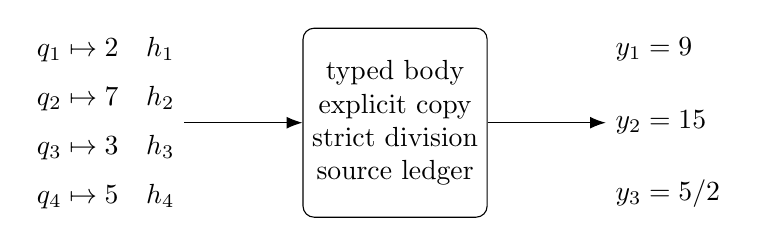
\begin{tikzpicture}[
  node distance=8mm and 15mm,
  box/.style={draw,rounded corners,align=center,minimum height=24mm},
  arr/.style={-{Latex[length=2mm]}}
]
\node[align=right] (inputs) {$q_1\mapsto2\quad h_1$\\[2mm]
$q_2\mapsto7\quad h_2$\\[2mm]$q_3\mapsto3\quad h_3$\\[2mm]
$q_4\mapsto5\quad h_4$};
\node[box,right=of inputs] (body) {typed body\\explicit copy\\strict division\\source ledger};
\node[align=left,right=of body] (outputs) {$y_1=9$\\[5mm]$y_2=15$\\[5mm]$y_3=5/2$};
\draw[arr] (inputs) -- (body);
\draw[arr] (body) -- (outputs);
\end{tikzpicture}
\caption{A fixed four-end AES carrier with four computational inputs and
three declared scalar outputs.  The diagram displays the program interface,
not paths of arithmetic gates through the AES.}
\label{fig:ported-four-inputs}
\end{figure}

Use either cut $|z-c|=3/4$ with $c=-1/2$ or $c=1/2$.  The inner and outer
charts on the overlap are
\[
  \xi=\frac{z-c}{3/4},\qquad
  \eta=\frac{3/4}{z-c},\qquad \eta=1/\xi.
\]
Each cut separates two marked ends from the other two.  For each cut, also
declare an allocation of gate occurrences to local packets; this allocation is
additional program data, not a consequence of the port anchoring map.
Restrict the carrier data to the chosen pieces and retain each local event
region, its exposed wire frontier, and the complete ordered seam/assembly
contract.
Reciprocal coordinate transport is an exact change of chart.  The tensor and
chain-rule argument in Proposition~\ref{prop:ported-collar-descent} recovers
the same global AES and operation network from either decomposition.  Local
seam source references identify transported data; they are not new constant
sources.  Execution after assembly follows the global event order, which need
not be a whole-piece block order.  No path of a binary gate through the AES
is asserted.

\subsection{Finite checks and remaining obligations}

The accompanying independent finite checker uses exact rational arithmetic for
this example and explicit positive and negative controls.  Its scope and
reproduction commands are recorded in the Paper~IV README.  It is a new
verification of the integrated model, not a rerun of the unavailable checker
reported with the candidate chapter.  Finite checks supplement the proofs;
they do not prove continuous collar identities or a faithful motion bridge.

The important negative controls are implicit sharing, duplicate binding,
mismatched types, unaccounted seam data, and cycles formed by locally acyclic
pieces.  A literal constant two and the producer $1+1$ have the same scalar
output but different sources and operation histories.  Strict evaluation
retains failure of a discarded $1/0$ producer.  Different association receipts
remain distinct, and Example~\ref{ex:feature-not-online} remains an obstruction
to online feature update.

The remaining obligations are stated as
Problems~\ref{prob:faithful-multiwire-aeg} and
\ref{prob:opposite-edge-features}: realize the actual typed generators by AES
state transformations and construct the actual opposite-edge feature
witnesses.  Neither is a consequence of finite program substitution.

\section{Operational resource geometry}\label{sec:operational-resources}
% Canonical Paper IV section.
Contextual residuals measure semantic distinguishability.  An execution uses
concrete data structures, schedules, memories, and communication links.  The
two layers meet only after a machine model says where a complete residual state
is represented.  The strict networks of Section~\ref{sec:ported-aes} supply one
concrete class of typed acyclic programs.  Their substitution theorem preserves
partial numerical semantics and provenance; it does not preserve the work,
storage, or scheduling cost of a chosen implementation.

\subsection{Logical cuts and live configurations}

Let $\Gamma$ be a typed acyclic computation network.  A logical cut separates
operations already licensed by causality from operations not yet licensed.  A
set of nodes that have ever been computed may record causal progress, but it
does not say which values are currently present.

\begin{definition}[Operational machine model]
An operational model $\cM$ specifies:
\begin{enumerate}
  \item the admissible input family and uniformity convention;
  \item value, instruction, and constant encodings;
  \item atomic compute, erase, move, communicate, checkpoint, and recompute
  actions;
  \item legal live configurations and their sizes;
  \item the cost of each action and the processor or memory topology;
  \item whether input, output, constants, tables, and code count toward space.
\end{enumerate}
\end{definition}

An execution is a legal trace
\begin{equation}
  L_0\xrightarrow{a_1}L_1\xrightarrow{a_2}\cdots
  \xrightarrow{a_T}L_T,
  \label{eq:live-configuration-trace}
\end{equation}
where $L_t$ lists the values and control records currently materialized.
Write $S_\sigma(t)=\operatorname{size}_{\cM}(L_t)$.

\begin{definition}[Resource vector]
For a realization $\Gamma$ and schedule $\sigma$, define
\begin{equation}
 \mathbf C_{\cM}(\Gamma,\sigma)
 =\bigl(
 L_{\mathrm{desc}},W,T,D_{\mathrm{caus}},S_{\max},\ST,Q
 \bigr),
 \label{eq:resource-vector}
\end{equation}
where
\[
 S_{\max}=\max_t S_\sigma(t),
 \qquad
 \ST=\sum_{t=0}^{T}S_\sigma(t).
\]
Here $L_{\mathrm{desc}}$ is static description size, $W$ weighted work,
$T$ scheduled time, $D_{\mathrm{caus}}$ intrinsic causal depth in the declared
parallel model, and $Q$ communication or I/O.
\end{definition}

These coordinates generally have different units.  A theorem comparing them
must state the simulation, charging, and encoding convention; adding them into
one scalar without such a rule has no invariant meaning.

\subsection{Why completed-node sets do not determine space}

\begin{theorem}[Completed-set insufficiency]
\label{thm:completed-set-insufficient}
Suppose a computation has a positive-size intermediate value that may legally
be retained or erased after its last immediate use.  Then the set of nodes ever
computed does not determine the current workspace.
\end{theorem}

\begin{proof}
Execute through the last use of the intermediate.  In one legal execution keep
its value; in another erase it.  The two executions have computed exactly the
same nodes, but their live configurations differ by a positive-size object.
\end{proof}

With recomputation the discrepancy is stronger: a value may disappear and
later be recreated while the ever-computed set remains unchanged.  Therefore a
monotone chain of down-sets cannot serve as a general pebble or checkpoint
state.

\begin{proposition}[Restricted frontier model]
\label{prop:restricted-frontier}
In a no-recomputation node-value model in which each value is retained exactly
until its last successor has executed, a down-closed completed set $I$ does
determine the live frontier
\[
  \partial^+ I
  =\{u\in I:\text{some successor of $u$ lies outside $I$}\}.
\]
If node $u$ occupies $b(u)$ units, then the corresponding workspace is
$\sum_{u\in\partial^+I}b(u)$, up to the separately declared input, output, and
control conventions.
\end{proposition}

The proposition remains useful, but only inside its restricted retention
policy.

\subsection{Embedding the residual lower bound}

A live configuration may carry much more than the minimal residual class.  It
may include redundant values, caches, checksums, code pointers, or a convenient
structured representation.  Nevertheless, when it is the complete exact online
state, it must distinguish residual classes.

\begin{proposition}[Live-state residual bound]
\label{prop:live-residual-bound}
At a cut $C$, suppose the charged live configuration contains a complete exact
state and is encoded either in a fixed-width $b$-bit slot or by a prefix-free
code of maximum length $b$.  Then
\[
  b\ge\left\lceil\log_2|\cR_C|\right\rceil.
\]
\end{proposition}

\begin{proof}
The live-state encoding is an exact online realization, so
Theorem~\ref{thm:minimal-exact-residual} maps its reachable states onto
$\cR_C$.  Apply the counting argument of
Corollary~\ref{cor:residual-bit-bound}.
\end{proof}

The following quantities must remain distinct:

\begin{center}
\begin{tabular}{L{0.25\textwidth}L{0.65\textwidth}}
\toprule
Quantity & Question answered\\
\midrule
$|\cR_C|$ & How many future behaviors remain semantically distinguishable?\\
$\lceil\log_2|\cR_C|\rceil$ & How many bits select one exact residual class in a fixed-width model?\\
$S_\sigma(t)$ & How large is the materialized configuration in this execution?\\
$L_{\mathrm{desc}}$ & How large is the program, circuit, table, or shared representation?\\
\bottomrule
\end{tabular}
\end{center}

A dense tensor with $D$ field entries, a low-rank factorization of the same
tensor, an index into a decision diagram, and the whole decision diagram are
four different representations.  Their sizes are not determined by the
cardinality of one abstract residual space.

\subsection{Uniform families and Pareto resource geometry}

Complexity belongs to input families rather than to one hard-coded finite map.
Let $F=(F_n)_{n\ge1}$ be a family and let
$\operatorname{Adm}^{\mathrm{unif}}_{\cM}(F)$ be the realization families
produced by one declared uniform constructor.  Define the fixed-size achievable
frontier
\begin{equation}
 \mathfrak C_{\cM}^{\mathrm{unif}}(F;n)
 =\Pareto\left\{
 \mathbf C_{\cM}(\Gamma_n,\sigma_n):
 ((\Gamma_j,\sigma_j))_{j\ge1}
 \in\operatorname{Adm}^{\mathrm{unif}}_{\cM}(F)
 \right\}.
 \label{eq:pareto-resource-geometry}
\end{equation}
Here $\Pareto$ retains nondominated vectors under coordinatewise comparison.
If limits are not attained, a closure may be needed.

Equation~\eqref{eq:pareto-resource-geometry} is a structural framework, not a
machine-independent invariant.  Its value changes with the model, units,
precision, uniformity, preprocessing, and allowed representations.  A robust
comparison across models would require explicit efficient simulations.

\subsection{Three distinct order effects}

The examples of this paper separate three phenomena:

\begin{center}
\begin{tabular}{L{0.25\textwidth}L{0.35\textwidth}L{0.28\textwidth}}
\toprule
Order effect & Meaning & Calibration\\
\midrule
semantic noncommutation & Order changes the induced operator or endpoint & affine add--scale histories\\
rewrite-plan variation & Semantics agree but factorization and costs differ & matrix-chain parenthesization\\
schedule or cut sensitivity & One computation exposes different live or residual widths & OBDD order and checkpointing\\
\bottomrule
\end{tabular}
\end{center}

Only the first already has the contact-curvature interpretation developed in
Paper~0~\cite{Yuan2026AEGPaperZero}.  The other two should not be called
curvature until a connection, gauge law, or $2$-cell defect has been supplied.

\section{Word growth, fibers, and information loss}\label{sec:growth-information}
% Canonical Paper IV section.
A quotient fiber can grow with word length, but cardinality, information, and
running time are different measurements.  This section records the exact
counting statements that survive without a machine model.

\subsection{Words, image growth, and fiber multiplicity}

Let $\Sigma$ be a finite alphabet with $s=|\Sigma|\ge2$.  For each $n$, let
\[
  \rho_n:\Sigma^n\longrightarrow Y_n
\]
be an evaluation or condensation map.  Define
\[
  N_n=|\rho_n(\Sigma^n)|,
  \qquad
  M_n=\max_{y\in Y_n}|\rho_n^{-1}(y)|.
\]

\begin{proposition}[Fiber--image inequality]
\label{prop:fiber-image-inequality}
For every $n$,
\begin{equation}
  M_n\ge \frac{s^n}{N_n}.
  \label{eq:fiber-image-inequality}
\end{equation}
\end{proposition}

\begin{proof}
The $s^n$ words are partitioned among $N_n$ nonempty fibers.  At least one
fiber has size at least the average.
\end{proof}

The inequality does not require a group, metric, or probability model.  It
shows only that small image growth forces some large history fiber.

\subsection{A conditional-information form}

Let $W_n$ be uniformly distributed on $\Sigma^n$ and put
$Y_n=\rho_n(W_n)$.  Shannon entropy is measured in bits~\cite{Shannon1948}.

\begin{proposition}[Evaluation information loss]
\label{prop:evaluation-information-loss}
One has
\begin{equation}
 H(W_n\mid Y_n)
 =n\log_2s-H(Y_n)
 \ge n\log_2s-\log_2N_n,
 \label{eq:conditional-information-loss}
\end{equation}
and
\[
  H(W_n\mid Y_n)\le\log_2M_n.
\]
\end{proposition}

\begin{proof}
Because $Y_n$ is a deterministic function of $W_n$,
$H(W_n,Y_n)=H(W_n)=n\log_2s$, while the chain rule gives
$H(W_n,Y_n)=H(Y_n)+H(W_n\mid Y_n)$.  Also
$H(Y_n)\le\log_2N_n$.  Conditional on $Y_n=y$, the word lies in a set of size
at most $M_n$, so its conditional entropy is at most $\log_2M_n$; averaging
preserves the bound.
\end{proof}

For a nonuniform distribution, the lost information depends on the fiber
weights, not only their cardinalities.  For an individual word, Kolmogorov or
description complexity would introduce another model and is not being used
here.

\subsection{Word metrics and coarse growth}

Let $G$ be a finitely generated group with finite symmetric generating set
$S$.  Write $|g|_S$ for word length and
\[
  \beta_S(n)=|\{g\in G:|g|_S\le n\}|.
\]

\begin{proposition}[Finite generating sets give comparable growth]
\label{prop:word-metric-comparison}
If $S$ and $T$ are finite generating sets, there are constants $A,B\ge1$ such
that
\[
  |g|_T\le A|g|_S,
  \qquad
  |g|_S\le B|g|_T
\]
for all $g\in G$.  Consequently
\[
  \beta_T(n)\le\beta_S(Bn),
  \qquad
  \beta_S(n)\le\beta_T(An).
\]
\end{proposition}

\begin{proof}
Every generator in one finite set is a bounded-length word in the other.  Let
$A$ and $B$ be the corresponding maximum lengths and substitute each letter in
a shortest word.
\end{proof}

Polynomial versus exponential group growth is therefore a coarse property of
the finitely generated group, not of one particular generating set.  Deep
structure theorems classify polynomial growth~\cite{Gromov1981}; the present
paper needs only the elementary comparison above.

\subsection{Four growth functions that must not be merged}

For a history language and evaluation map one may encounter:
\begin{align*}
  W(n)&=\#\{\text{literal words of length at most }n\},\\
  N_\rho(n)&=\#\{\text{distinct evaluated operators reached by those words}\},\\
  M_\rho(n)&=\max_g\#\{\text{words of length at most }n\text{ evaluating to }g\},\\
  R_C(n)&=\#\{\text{contextual residual classes exposed at a selected cut}\}.
\end{align*}
A search algorithm adds still another quantity: the number of states it
actually explores under a specified strategy.  None of these functions is the
running time by definition.

\begin{example}[Free reduction]
The ball of radius $n$ in a free group of rank at least two grows
exponentially, but a given word can be freely reduced by a stack in time linear
in its input length.  Exponential group growth therefore does not imply
exponential evaluation time.
\end{example}

\begin{example}[Finite projective image]
For fixed $q$, every sufficiently long bilateral word over a finite generating
alphabet evaluates into the finite group $\PGL_2(\F_q)$.  Literal word counts
continue to grow, while $N_\rho(n)$ eventually saturates at at most
$q(q^2-1)$.  The growing fibers measure many realizations of a finite semantic
state, not unbounded state-space size.
\end{example}

\subsection{Geometry requires a comparison map}

Hyperbolic spaces and many groups have exponential ball growth.  A history
language may also have exponential word growth.  Equality of the adjectives
``exponential'' does not provide a quasi-isometry, coding theorem, or
simulation.  A geometric complexity theorem would need at least:

\begin{enumerate}
  \item a map from histories or live states into the geometric space;
  \item upper and lower distortion estimates for the selected metrics;
  \item a simulation relating geometric steps to machine actions;
  \item a representation theorem linking geometric volume to encoded states.
\end{enumerate}

Without these data, curvature and volume remain motivating analogies.  The
fixed-model identities in the case studies below are not promoted to a general
curvature--complexity law.

\section{Rewrite fibers, normal forms, and exactness obstructions}\label{sec:rewrite-fibers}
% Canonical Paper IV section.
Evaluation fibers contain realizations with equal semantics.  A rewrite system
organizes paths inside such a fiber.  The cost of traversing a rewrite path,
the distance between two realizations, the filling of a coherence loop, and a
possible holonomy are distinct structures.

\subsection{Rewrite graphs and normal forms}

Let $X$ be a set of realizations and $\rho:X\to Y$ their semantics.  For
$y\in Y$, write
\[
  \mathcal F_y=\rho^{-1}(y).
\]
A semantics-preserving rewrite relation $\mathcal R$ has directed edges
$x\to x'$ only when $\rho(x)=\rho(x')$.  It therefore decomposes into graphs
on the fibers $\mathcal F_y$.

\begin{definition}[Rewrite distance and filling]
For two vertices in the same undirected rewrite component, let
$d_\mathcal R(x,x')$ be the shortest number or declared weight of rewrite
edges connecting them.  If rewrite relations are supplied as $2$-cells, let
$\Fill_\mathcal R(\ell)$ be the minimum number or weight of $2$-cells filling
a closed rewrite loop $\ell$, when such a filling exists.
\end{definition}

A terminating and confluent rewrite system selects a unique normal form in
each connected semantic class.  Termination plus local confluence is sufficient
for confluence by Newman's lemma~\cite{Newman1942}.  A normal form may make
equality testing efficient, but its construction cost and output size still
require a computational model.

\subsection{Potential labels are exact}

Let $A$ be an additive abelian group and let $C:X\to A$ be any single-valued
potential, for example a cost assigned to a completed realization.

\begin{proposition}[Additive exactness obstruction]
\label{prop:additive-exactness-obstruction}
If a rewrite edge is labelled
\[
  \omega_C(x\to x')=C(x')-C(x),
\]
then every finite closed rewrite loop satisfies
\[
  \sum_{e\in\ell}\omega_C(e)=0.
\]
\end{proposition}

\begin{proof}
The sum telescopes; every intermediate potential occurs once with each sign,
and the initial and terminal vertices coincide.
\end{proof}

The same obstruction holds noncommutatively for pure-gauge labels.

\begin{proposition}[Group-valued pure-gauge obstruction]
\label{prop:pure-gauge-obstruction}
Let $h:X\to L$ take values in a group and label an edge by
\[
  r(x\to x')=h(x')h(x)^{-1}.
\]
With chronological multiplication, the ordered product around every closed
loop is the identity.
\end{proposition}

\begin{proof}
For a path $x_0\to x_1\to\cdots\to x_m$, the chronological product is
\[
 r(x_{m-1}\to x_m)\cdots r(x_0\to x_1)
 =h(x_m)h(x_0)^{-1}.
\]
The factors cancel successively.  On a closed loop $x_m=x_0$, this is the
identity.
\end{proof}

These propositions apply to endpoint-potential differences on an associahedron
and to the exact frame transport of
Proposition~\ref{prop:exact-transport-telescope}.  They do not say that every
connection is flat; they say that a globally exact label cannot certify
nontrivial holonomy.

\subsection{Action is not holonomy}

A closed rewrite plan may have positive accumulated work even when its exact
potential sum and pure-gauge product vanish.  Work charges actions, whereas
holonomy compares transported frames after quotienting by gauge.  Calling
positive loop work ``curvature'' would erase this distinction.

For a weighted directed rewrite path
$x=x_0\to x_1\to\cdots\to x_m=x'$, define
\[
  \operatorname{Act}(x_\bullet)=\sum_{i=0}^{m-1}c(x_i\to x_{i+1}),
  \qquad c\ge0.
\]
Even when $x=x'$, the action can be positive.  This records dissipation or work
under the selected rewriting algorithm, not a group-valued failure of exact
transport.

\subsection{Large fibers can have shared representations}

A semantic fiber may contain exponentially many words while admitting a small
DAG, grammar, circuit, or congruence-closed representation that shares common
substructure.  Conversely, a small semantic set can require large intermediate
objects in a restricted representation language.  Therefore
\[
  |\mathcal F_y|\ \text{large}
  \quad\not\Longrightarrow\quad
  L_{\mathrm{desc}}\ \text{large}
\]
without a lower-bound theorem for the chosen representation class.

The case studies make the separation concrete:

\begin{itemize}
  \item Horner words have an exactly countable charge fiber of distinct
  operators;
  \item OBDDs share equal residual functions but can still have exponentially
  different widths under different variable orders;
  \item matrix-chain parenthesizations are vertices of an associahedral
  rewrite fiber with different arithmetic costs;
  \item checkpoint schedules realize one derivative computation with different
  live-state traces.
\end{itemize}

\subsection{The non-exact transport problem}

A future projective rewrite geometry would need:

\begin{enumerate}
  \item a category or $2$-category of histories and semantics-preserving
  rewrites;
  \item an edge transport not forced to be an endpoint coboundary;
  \item a gauge transformation law and a class of coherence $2$-cells;
  \item at least one closed loop with a gauge-invariant nontrivial residue;
  \item a comparison with the affine torsion of Paper~0 on the Borel sector.
\end{enumerate}

Until these conditions are met, rewrite distance and filling are legitimate
geometric quantities, while ``projective rewrite curvature'' remains an open
programme.

\section{Horner histories and ACS condensation}\label{sec:horner}
% Canonical Paper IV section.
The first calibration stays inside the affine sector of AEG.  It shows exactly
how a commutative charge shadow can forget positional information while the
evaluated operators remain distinct.

\subsection{Radix histories}

Fix an integer radix $k\ge2$ and the digit alphabet
$D_k=\{0,1,\ldots,k-1\}$.  For $d\in D_k$, let
\[
  h_d(x)=kx+d.
\]
A chronological word $w=d_1d_2\cdots d_n$ acts by
\[
  \rho(w)=h_{d_n}\circ\cdots\circ h_{d_1}.
\]

\begin{proposition}[Horner evaluation formula]
\label{prop:horner-evaluation}
For every length-$n$ word,
\begin{equation}
  \rho(w)(x)
  =k^n x+\sum_{i=1}^{n}d_i k^{n-i}.
  \label{eq:horner-evaluation}
\end{equation}
\end{proposition}

\begin{proof}
Induction on $n$.  Appending $d_{n+1}$ sends the current value $y$ to
$ky+d_{n+1}$, multiplying all previous coefficients by $k$ and adding the new
least significant digit.
\end{proof}

\begin{theorem}[Radix-word injectivity]
\label{thm:radix-word-injectivity}
Over $\Z$, or over a characteristic-zero field containing the displayed
integers, distinct words in $D_k^n$ induce distinct affine operators.
\end{theorem}

\begin{proof}
All operators have slope $k^n$.  Equality would force equality of the constants
in Equation~\eqref{eq:horner-evaluation}.  These constants are the integers
$0,1,\ldots,k^n-1$ written uniquely in length-$n$ base-$k$ notation, allowing
leading zeros.
\end{proof}

The characteristic-zero hypothesis is active.  Over a finite field, distinct
integer constants may coincide after reduction; Section~\ref{sec:butterfly-ntt}
uses such modular identification deliberately.

\subsection{Condensation by ACS charge}

Realize $h_d$ as a scale by $k$ followed by an addition of $d$.  The ACS of
Paper~0~\cite{Yuan2026AEGPaperZero} records only total additive and
logarithmic multiplicative charge.  Hence
\begin{equation}
  \chi(w)=\left(\sum_{i=1}^{n}d_i,\ n\log k\right).
  \label{eq:horner-charge}
\end{equation}

\begin{theorem}[Fixed-histogram operator count]
\label{thm:horner-histogram-count}
Let $m_r$ be the number of occurrences of digit $r$, with
$\sum_{r=0}^{k-1}m_r=n$.  All words with this histogram have the same ACS
charge, and they induce exactly
\begin{equation}
  \frac{n!}{\prod_{r=0}^{k-1}m_r!}
  \label{eq:multinomial-horner-count}
\end{equation}
distinct affine operators.
\end{theorem}

\begin{proof}
Equation~\eqref{eq:horner-charge} depends only on the histogram.  The number of
words with the histogram is the multinomial coefficient.  They give distinct
operators by Theorem~\ref{thm:radix-word-injectivity}.
\end{proof}

\begin{corollary}[Binary fixed-weight fiber]
\label{cor:binary-horner-count}
For $k=2$, the length-$n$ words with exactly $m$ ones have one ACS charge and
$\binom nm$ distinct operator images.  Under the uniform distribution on that
set, conditioning only on the charge loses
\[
  \log_2\binom nm
\]
bits of word information.
\end{corollary}

For $n=4$ and $m=2$, the six constants are
\[
  3,5,6,9,10,12,
\]
corresponding to the six placements of two ones.  The charge remembers their
number but not their positions.

\subsection{Which state is sufficient?}

For all future affine continuations, the current affine operator is sufficient:
composition depends only on its slope and translation.  The ACS charge is not
sufficient, because two words with one charge can already have different
translations before any future is applied.  If the observation is deliberately
coarsened to ACS charge and all future updates act only on charge, then the
charge becomes an exact residual for that smaller experiment.

This illustrates the hierarchy
\[
  \text{word}
  \longrightarrow
  \text{affine operator}
  \longrightarrow
  \text{ACS charge}.
\]
The size in Theorem~\ref{thm:horner-histogram-count} is the operator image of a
charge fiber.  It is not a fiber of operator evaluation.

\subsection{Streaming cost and encoding cost}

The recurrence
\[
  a_i=ka_{i-1}+d_i
\]
evaluates a word in $n$ affine steps while storing one current field element.
In a unit-cost field-operation model this is $O(n)$ work and $O(1)$ field
elements of workspace.  Over the integers, however, the bit length of $a_i$
is $\Theta(i\log k)$ in the worst case.  Thus ``one accumulator'' does not mean
constant bit space in a bit-complexity model.

The example therefore supplies an exact condensation count but no generic
search or hardness theorem.  Positional information can be large while direct
streaming evaluation remains simple.

\section{Cut order and residual width in decision diagrams}\label{sec:obdd}
% Canonical Paper IV section.
Ordered binary decision diagrams give a finite model in which contextual
residual classes are represented directly as graph nodes.  The example also
shows that exponential cut sensitivity does not require noncommuting semantic
operations.

\subsection{Residual functions after a variable prefix}

Let $F:\{0,1\}^N\to\{0,1\}$ and fix a variable order $\pi$.  After assigning
the first $t$ variables according to a prefix $\alpha$, the remaining behavior
is the restricted function $F|_\alpha$.

\begin{proposition}[Residual-width lower bound]
\label{prop:obdd-residual-lower-bound}
Every deterministic OBDD respecting $\pi$ has, at the cut after the first $t$
variables, at least as many distinct reachable nodes as there are distinct
restricted functions $F|_\alpha$.
\end{proposition}

\begin{proof}
If two prefixes reach the same node, every common continuation follows the same
remaining subgraph and therefore gives the same Boolean answer.  Hence the two
restricted functions are equal.  Distinct residual functions must reach
distinct nodes.
\end{proof}

For reduced OBDDs the converse also holds: isomorphic remaining subfunctions
are merged.  This is the decision-diagram instance of
Theorem~\ref{thm:minimal-exact-residual}; see~\cite{Bryant1986,Wegener2000}.

\subsection{Equality under block order}

Define
\[
  \operatorname{EQ}_n(x,y)=1
  \quad\Longleftrightarrow\quad
  x=y,
  \qquad x,y\in\{0,1\}^n.
\]
Consider the block order
\[
  x_1,\ldots,x_n,y_1,\ldots,y_n.
\]
After all $x$-variables have been assigned to a string $a$, the residual
function is
\[
  g_a(y)=\mathbf1[y=a].
\]

\begin{theorem}[Exponential middle width]
\label{thm:eq-block-width}
Every OBDD for $\operatorname{EQ}_n$ in block order has width at least $2^n$
at the middle cut.
\end{theorem}

\begin{proof}
The functions $g_a$, $a\in\{0,1\}^n$, are pairwise distinct.  Apply
Proposition~\ref{prop:obdd-residual-lower-bound}.
\end{proof}

The logarithm of this width is $n$ bits, exactly the information needed to
remember the first block for arbitrary comparison with the second.

\subsection{Equality under interleaved order}

Now use
\[
  x_1,y_1,x_2,y_2,\ldots,x_n,y_n.
\]
While equality has not failed, reading $x_i$ creates one of two pending states,
``the next $y_i$ must be $0$'' or ``the next $y_i$ must be $1$''.  Reading
$y_i$ returns to the matching state or goes permanently to the zero terminal.

\begin{theorem}[Constant interleaved width]
\label{thm:eq-interleaved-width}
There is an OBDD for $\operatorname{EQ}_n$ in interleaved order with maximum
width at most three and total size $O(n)$.
\end{theorem}

\begin{proof}
Use the matching state, the two pending-bit states, and the shared zero
terminal as described above.  At any variable level at most three nonterminal
or active residual states are needed, and each pair of variables contributes
only a constant number of nodes.
\end{proof}

The two orders therefore expose exponentially different residual widths for
the same Boolean function and representation language.

\subsection{The restrictions commute}

Assignments to two distinct variables commute as semantic restriction
operators:
\[
  (F|_{x_i=a})|_{x_j=b}
  =(F|_{x_j=b})|_{x_i=a}.
\]
Nevertheless, the order in which variables cross the cut changes which partial
information must remain available.  The exponential separation in
Theorems~\ref{thm:eq-block-width} and
\ref{thm:eq-interleaved-width} is therefore a schedule and representation
phenomenon, not a consequence of operator noncommutativity.

\subsection{What the width theorem measures}

At one cut, $\log_2(\text{width})$ lower-bounds the number of bits needed to
select a residual node.  The entire OBDD also stores transitions for all input
prefixes, so its static node count is a different resource.  Moreover, a
program outside the OBDD model might compute equality with a different state
organization.  The theorem is exact for fixed variable order and the OBDD
representation class; it is not a model-independent lower bound for every
algorithm computing equality.

\section{Butterflies, transform representations, and NTT states}\label{sec:butterfly-ntt}
% Canonical Paper IV section.
Fast transforms illustrate representation change rather than endpoint
shortcuts.  A local butterfly has a precise projective quotient description,
but a full transform is a multi-wire linear network and must retain data that
one-wire projective semantics discards.

\subsection{The butterfly torus-coset lemma}

Let $K$ be a field with $\operatorname{char}K\ne2$ and let
$\omega\in K^\times$.  Define
\[
  \mathsf B_\omega=
  \begin{pmatrix}1&\omega\\1&-\omega\end{pmatrix},
  \qquad
  \mathsf B_1=
  \begin{pmatrix}1&1\\1&-1\end{pmatrix},
  \qquad
  D_\omega=
  \begin{pmatrix}1&0\\0&\omega\end{pmatrix}.
\]

\begin{proposition}[Butterfly torus coset]
\label{prop:butterfly-coset}
In $\GL_2(K)$,
\begin{equation}
  \mathsf B_\omega=\mathsf B_1D_\omega.
  \label{eq:butterfly-factorization}
\end{equation}
After projectivization, if $H$ is the diagonal stabilizer of
$(0,\infty)$, then
\[
  \mathsf B_\omega H=\mathsf B_1H.
\]
Thus all nonzero twiddle butterflies have one quotient skeleton and a
lift-dependent diagonal label.
\end{proposition}

\begin{proof}
Equation~\eqref{eq:butterfly-factorization} is direct multiplication, and
$D_\omega\in H$ after projectivization.  The determinant
$-2\omega$ is nonzero under the hypotheses.
\end{proof}

This is a right-$H$-coset statement.  It does not identify the two-wire gate
with a one-hole arithmetic context, nor does it make the diagonal coordinate a
canonical gauge-independent residue.

\subsection{Why linear-group data remain necessary}

The inverse is
\[
  \mathsf B_\omega^{-1}
  =\frac12
  \begin{pmatrix}1&1\\\omega^{-1}&-\omega^{-1}\end{pmatrix}.
\]
Projectivization forgets the common scalar, but exact inverse transforms and
integer or finite-field arithmetic must retain normalization factors.  A full
FFT or NTT therefore belongs naturally to a linear multi-wire category with
objects $K^N$, not solely to $\PGL_2(K)$.

\begin{construction}[Network AEG interface]
A prospective multi-wire extension would have wire arities as objects,
linear or arithmetic gates as morphisms, tensor product as parallel
composition, and ordinary composition as layer gluing.  It should contain the
one-wire marked histories as a subcategory and admit a semantics functor to
maps $K^m\to K^n$.
\end{construction}

This construction is a structural proposal.  Proposition~\ref{prop:butterfly-coset}
is the proved local interface.

\subsection{Transform factorization of convolution}

For a field containing a primitive $N$-th root of unity and with $N$ invertible,
the discrete Fourier transform $F_N$ converts cyclic convolution into
pointwise multiplication:
\begin{equation}
  x*y
  =F_N^{-1}\bigl(F_Nx\odot F_Ny\bigr).
  \label{eq:convolution-transform}
\end{equation}
Radix factorizations reduce the transform from a dense matrix-vector product to
$O(N\log N)$ local butterflies in the standard algebraic operation model; the
classical radix-two algorithm is due to Cooley and Tukey~\cite{CooleyTukey1965}.

For $N=2^m$, a fixed breadth-first radix-two network has
\begin{equation}
  D_{\mathrm{net}}=m,
  \qquad
  W_{\mathrm{cell}}=\frac N2m
  \label{eq:radix2-network-counts}
\end{equation}
synchronous layers and butterfly cells, respectively.

Integer multiplication requires more than
Equation~\eqref{eq:convolution-transform}: coefficient encoding, padding or a
noncyclic construction, carry recovery, sufficiently large moduli or CRT, and
bit-complexity analysis must also be charged.

\subsection{A finite NTT calibration}

Take $K=\F_{257}$.  Fermat's theorem gives $3^{256}=1$, while direct repeated
squaring gives
\[
  3^{128}=-1\pmod{257}.
\]
Hence $3$ has order $256$.  For $N\mid256$ put
\[
  \zeta_N=3^{256/N};
\]
then $\zeta_N$ is a primitive $N$-th root.  In particular,
$\zeta_8=64$ and $\zeta_{16}=249$.

\begin{proposition}[Layer-state count]
\label{prop:ntt-layer-states}
Let a fixed radix-two NTT layer be invertible on $\F_{257}^N$ and let the input
range be all of $\F_{257}^N$.  Then the reachable state set at that layer has
exactly $257^N$ elements.  Its logarithmic cardinality is
$N\log_2 257$ bits, while the direct fixed-width encoding by residues
$0,\ldots,256$ uses $9N$ bits.
\end{proposition}

\begin{proof}
An invertible layer is a bijection of $\F_{257}^N$, so its image is the whole
space.  Cardinality and the two encodings follow immediately.
\end{proof}

For $N=8$ the network has three layers and twelve butterflies; for $N=16$ it
has four layers and thirty-two butterflies.

\subsection{Static labels versus dynamic states}

A fixed transform's twiddle factors are program constants.  They may be stored
in a table, represented by a primitive root and exponent schedule, or generated
on demand.  Their storage--reconstruction tradeoff concerns
$L_{\mathrm{desc}}$, work, and perhaps cache traffic.  It is not dynamic input
entropy.  Conversely, the $N$ wire values vary with the input and belong to the
live state.

The safe representation principle is therefore:

\begin{quote}
Seek a declared change of representation in which the core operation is
diagonal, block-diagonal, sparse, or low-bandwidth, while charging the forward
transform, inverse transform, static constants, numerical precision, and
communication.
\end{quote}

This principle motivates AEG-native representation search, but it is not a
definition of every fast algorithm and does not prove an asymptotic improvement
by itself.

\section{Equal semantics with different work and space}\label{sec:time-space}
% Canonical Paper IV section.
The preceding examples varied semantic quotients and cut order.  We now keep
the final map fixed and vary its realization.  Matrix parenthesization changes
arithmetic work and intermediate shape; reverse-mode checkpointing exchanges
stored history for recomputation.

\subsection{Matrix-chain parenthesization}

Let
\[
  A\in K^{d_0\times d_1},
  \qquad B\in K^{d_1\times d_2},
  \qquad C\in K^{d_2\times d_3}.
\]
Both $(AB)C$ and $A(BC)$ evaluate to the same linear map whenever the products
are defined.

\begin{proposition}[Three-matrix work and principal intermediates]
\label{prop:matrix-chain-costs}
Under ordinary dense multiplication, counting scalar multiplications,
\[
  W_L=d_0d_1d_2+d_0d_2d_3,
  \qquad
  R_L=d_0d_2,
\]
\[
  W_R=d_1d_2d_3+d_0d_1d_3,
  \qquad
  R_R=d_1d_3,
\]
where $R_L$ and $R_R$ are the numbers of scalar entries in the principal
intermediate matrices $AB$ and $BC$.
\end{proposition}

\begin{proof}
Multiplying an $r\times s$ matrix by an $s\times t$ matrix uses $rst$ scalar
multiplications in the stated algorithm and produces an $r\times t$ matrix.
Apply this twice in each order.
\end{proof}

For $(d_0,d_1,d_2,d_3)=(100,10,1,2)$,
\[
  (W_L,R_L)=(1200,100),
  \qquad
  (W_R,R_R)=(2020,20).
\]
The lower-work plan has the larger principal intermediate.  The $R$ values are
not complete peak-memory formulas: input retention, output allocation,
overwrite policy, blocking, and temporaries still need to be declared.

For four matrices, the five parenthesizations form the vertices of an
associahedral pentagon.  If an edge is labelled by the difference of endpoint
costs, Proposition~\ref{prop:additive-exactness-obstruction} makes its sum around
the pentagon zero.  Positive work spent traversing the pentagon is action, not
holonomy.

\subsection{A chain and its reverse sweep}

Consider a length-$N$ composition
\[
  x_{i+1}=f_i(x_i),
  \qquad 0\le i<N,
\]
and its reverse accumulation
\[
  \bar x_i=Df_i(x_i)^*\bar x_{i+1}.
\]
The reverse step requires the corresponding forward state $x_i$.

Assume each forward evaluation and each reverse local step has unit cost and
each state has fixed size.

\begin{proposition}[Two exact endpoint schedules]
\label{prop:reverse-chain-extremes}
The following schedules compute the same reverse result.
\begin{enumerate}
  \item Store all forward states.  The total local work is $2N$ and the number
  of stored forward states is $\Theta(N)$.
  \item Store only the input and recompute each required prefix.  The total
  local work is
  \begin{equation}
    2N+\frac{N(N-1)}2,
    \label{eq:naive-recompute-work}
  \end{equation}
  and only $\Theta(1)$ states need be live, apart from the declared input,
  output, and control records.
\end{enumerate}
\end{proposition}

\begin{proof}
The store-all schedule performs $N$ forward and $N$ reverse local operations.
For the second schedule, the initial forward pass still costs $N$, the reverse
steps cost $N$, and reconstructing $x_i$ from $x_0$ costs $i$ forward steps.
Summing $i=0,\ldots,N-1$ gives Equation~\eqref{eq:naive-recompute-work}.
\end{proof}

Checkpointing interpolates between these extremes.  Under a specified number
of checkpoints and a uniform linear chain, schedules such as
\textsc{Revolve} optimize the recomputation pattern for their declared model
and objective~\cite{GriewankWalther2000}.

\subsection{History condensation and re-expansion}

A checkpoint is a materialized summary of the forward history sufficient to
restart from that point.  Erasing it condenses the live trace further;
recomputation re-expands the missing segment from an earlier checkpoint.  This
interpretation is structurally compatible with AEG's process-before-result
principle, but it does not identify a nonlinear derivative pullback with one
global projective inverse.

The example validates the live-configuration correction of
Theorem~\ref{thm:completed-set-insufficient}.  Both schedules eventually compute
the same forward nodes and the same reverse result, yet their live states and
work differ.  No monotone set of ever-computed nodes can encode that tradeoff.

\subsection{Reversible computation boundary}

A logically reversible realization must retain or reconstruct information that
a many-to-one step would otherwise erase.  General reversible simulations
therefore exhibit time--space tradeoffs; Bennett's pebbling construction is a
classical model~\cite{Bennett1989}.  The present paper uses this as an external
calibration, not as a theorem that every AEG condensation has the same optimal
tradeoff.

\subsection{What equal semantics permits us to conclude}

Matrix chains and checkpoint schedules prove that one semantic map can have
incomparable resource vectors.  They support the Pareto viewpoint of
Equation~\eqref{eq:pareto-resource-geometry}.  They do not show that all time
and space costs are coordinates of one scalar ``representation volume.''  A
unification would require a model-specific theorem relating semantic residuals,
live encodings, and allowed re-expansions.

\section{Claim boundaries and the remaining programme}\label{sec:boundaries}
% Canonical Paper IV section.
The preceding sections prove a collection of comparison theorems, not a
universal complexity law.  This section gathers the claim boundary in one
place and formulates the remaining AEG programme in falsifiable terms.

\subsection{The four layers}

The completed framework distinguishes:
\begin{equation}
\boxed{
\begin{array}{c}
\text{projective quotient fibers}\\[1mm]
\Hist_K\to G\to G/H\to G/B_\pm
\end{array}}
\qquad
\boxed{
\begin{array}{c}
\text{contextual residuals}\\[1mm]
(P_C,M_C,O_C)\mapsto\cR_C
\end{array}}
\label{eq:four-layer-first-pair}
\end{equation}
\begin{equation}
\boxed{
\begin{array}{c}
\text{operational live configurations}\\[1mm]
(\cM,\Gamma,\sigma)\mapsto\mathbf C_\cM
\end{array}}
\qquad
\boxed{
\begin{array}{c}
\text{rewrite fibers}\\[1mm]
\rho^{-1}(y),\mathcal R\mapsto d_\mathcal R,\Fill_\mathcal R
\end{array}}.
\label{eq:four-layer-second-pair}
\end{equation}

The projective fiber is algebraic.  The contextual residual is semantic and
future-relative.  The live configuration is machine-dependent and dynamic.
The rewrite fiber organizes equal semantic realizations.  The paper proves
bridges only when the required actions and observations have been supplied.

\subsection{Principal proved statements}

\begin{center}
\begin{longtable}{L{0.16\textwidth}L{0.46\textwidth}L{0.27\textwidth}}
\toprule
Layer & Proved statement & Active boundary\\
\midrule
\endfirsthead
\toprule
Layer & Proved statement & Active boundary\\
\midrule
\endhead
projective & Regular bivaluations are rank-one idempotents and form $G/H$; projective frames form an $H$-torsor. & No canonical connection or semantic interpretation of a projector is inferred.\\
continuation & Left futures descend to $G/H$; one right update descends iff $k^{-1}Hk\subseteq H$; reversible right action requires the normalizer. & The conclusion depends on chronology and the selected quotient observation.\\
residual & $\cR_C$ is the canonical minimal exact deterministic state; finite residuals give a fixed-width bit lower bound. & Randomized, approximate, infinite, and lossy models require new definitions.\\
ported programs & Strict finite substitution preserves sources and occurrences and commutes with evaluation on the exact composite domain; compatible collars and interfaces descend. & Global DAG, complete seam records, strict partial domains; no AES gate-motion realization is inferred.\\
features & Observation factorization holds iff feature fibers refine contextual equivalence; online updates hold iff the feature kernel is a right congruence. & Observation factorization, effectiveness, and actual opposite-edge witnesses are separate obligations.\\
operational & Live configurations, not ever-computed sets, determine workspace when erase or recompute actions exist. & Actual resources remain model-, encoding-, and schedule-dependent.\\
growth & Fiber--image and conditional-entropy inequalities are exact. & Word growth and fiber growth are not running-time lower bounds.\\
rewrite & Potential differences and pure-gauge labels telescope on closed loops. & Nontrivial holonomy needs non-exact transport and a gauge law.\\
Horner & A fixed digit histogram has a multinomial number of distinct operators with one ACS charge in characteristic zero. & The count is not a hardness result and can collide in finite characteristic.\\
OBDD & Equality has exponential block-order width and constant interleaved-order width. & This is a representation- and order-specific theorem.\\
transform & Butterflies occupy one projective torus coset; radix networks have exact layer and cell counts. & A full FFT/NTT is multi-wire $\GL$ data with scalar, precision, and communication costs.\\
time--space & Matrix chains and checkpoint schedules give equal semantics with incomparable resource vectors. & No machine-independent scalar unifies the coordinates.\\
\bottomrule
\end{longtable}
\end{center}

The detailed hypothesis ledger appears in Appendix~\ref{app:ledger}.

\subsection{Excluded implications}

The following implications are neither proved nor used:
\[
  \text{noncommutativity}\Longrightarrow\text{negative curvature},
  \qquad
  \text{negative curvature}\Longrightarrow\text{algorithmic hardness},
\]
\[
  \text{exponential group growth}\Longrightarrow\text{exponential evaluation time},
\]
\[
  \text{large history fiber}\Longrightarrow\text{large shared representation},
  \qquad
  \text{endpoint cost difference}\Longrightarrow\text{holonomy}.
\]
Counter-calibrations occur inside the paper: free reduction is linear despite
exponential free-group growth; OBDD order can create exponential width although
variable restrictions commute; exact edge potentials telescope; and one
streaming Horner accumulator evaluates a charge fiber containing many distinct
operators.

\subsection{Interfaces with Papers 0--III}

Paper~I supplies marked spinal histories and bilateral projective evaluation
\cite{Yuan2026AEGFoundations}; Paper~0 supplies the affine/Borel sector, ACS
charge, torsion, and contact curvature \cite{Yuan2026AEGPaperZero}.  Paper~IV
imports those objects but does not
rewrite their foundational proofs.  The quotient tower and residual theory
begin after operator evaluation.

Paper~II supplies analytic representations and finite affine--Appell families
\cite{Yuan2026AEGFunctionTheory}.  They motivate the search for coordinates in
which selected operators become sparse or triangular.  Paper~IV does not claim
function-space completeness or a new asymptotically fast transform from those
families.

Paper~III supplies singular zero networks, arithmetic register fibers,
monodromy, and explicit forgetting phenomena~\cite{Yuan2026AEGZeroGeometry}.
Those examples demonstrate that finite forgetting maps can lose geometric
information.  Paper~IV does not identify the Lyashko--Looijenga forgetting
variance, braid monodromy, or tube energy with computational complexity.

The dependency remains one-way:
\[
  \text{Papers I--III provide typed examples}
  \longrightarrow
  \text{Paper IV supplies quotient and resource comparisons}.
\]

\subsection{Open problems}

The projective-torsion problem stated in earlier versions of this section is
resolved in the main text and is no longer listed here.  The
incidence-coupled transport of
Definition~\ref{def:projective-edge-transport} reduces to the affine cocycle on
the Borel sector and carries the non-telescoping cross-ratio holonomy
$\Lambda(\square)$ of Theorem~\ref{thm:projective-torsion-solution}; a finite
witness is given in Example~\ref{ex:f7-cross-ratio-holonomy}.  What remains open
there is not the existence of the comparison but its \emph{normalisation}: the
first-order density of the transport and the curvature of the reductive
connection of Remark~\ref{rem:reductive-connection} differ by a factor of two,
and no invariant currently fixes which normalisation a further application
should use.

\begin{problem}[Projective-to-contextual bridge]
Classify continuation experiments for which an $H$-lift, a quotient point
$gH$, or a conjugacy class of relative defects is a complete contextual
residual.  Determine sharp refinements when right and left futures are both
allowed.
\end{problem}

\begin{problem}[Faithful multi-wire AES realization]
\label{prob:faithful-multiwire-aeg}
Extend the finite ported-network interface of Section~\ref{sec:ported-aes} to a
symmetric monoidal category or PROP with a faithful AES state realization.
Supply a multi-hole configuration or fiber carrier and realize the actual typed
arithmetic and structural generators, including binary gates, copy, discard,
and their ordinary domains.  Retain sources, occurrences, literal call receipts,
and full-state residuals.  Prove execution transport, overlap conjugacy, and
independence of decomposition.  Recover the marked-history one-wire fragment
and a linear sector containing butterfly networks, retaining central scalars.
The finite attached-network theorem settles neither these geometric
realizations nor these embedding requirements.
\end{problem}

\begin{problem}[Opposite-edge feature witnesses]
\label{prob:opposite-edge-features}
Construct the actual three characteristic witnesses in a declared Adva
experiment \cite{Yuan2026AdvaArithmeticCalibration}.  Determine whether they
satisfy Theorem~\ref{thm:feature-observation-descent} and
Proposition~\ref{prop:feature-online-update}, or which retained process data
are needed to refine them.  Declare operator closure before using spectra and
snapshot/update or fixed-point semantics before using three-side feedback.
The scalar outputs in Example~\ref{ex:ported-four-puncture} do not identify
these native output roles.
\end{problem}

\begin{problem}[Costed representation change]
For a declared transform class $\Phi$, define and analyze
\[
  \cC(F;\Phi)
  =\cC(\Phi)+\cC(\Phi F\Phi^{-1})+\cC(\Phi^{-1})
\]
with precision, conditioning, static constants, communication, and uniformity
included.  Exhibit an AEG-native family for which the optimized representation
provably improves a baseline model.
\end{problem}

\begin{problem}[Approximate residuals]
Replace exact equality in Definition~\ref{def:contextual-equivalence} by a
metric, probabilistic, or decision-theoretic tolerance.  Determine which
covering, packing, mutual-information, or rate--distortion quantities replace
$\log_2|\cR_C|$.
\end{problem}

\begin{problem}[History-natural cost functor]
Construct a functor from a typed history or network category to a resource
category that records legal simulation, composition, erasure, and
recomputation.  Prove which resource coordinates are subadditive, additive, or
monotone under composition.
\end{problem}

\begin{problem}[Model robustness]
Identify a class of machine models connected by efficient simulations for which
the Pareto geometry in Equation~\eqref{eq:pareto-resource-geometry} is stable up
to declared distortions.
\end{problem}

\begin{problem}[Rosetta graph families]
Use chains, trees, diamonds, grids, and butterflies as common graph topologies
for expression evaluation, proof search, tensor contraction, differentiation,
and transforms.  Determine which residual and resource quantities are graph
invariants and which depend essentially on values, futures, or representations.
\end{problem}

These problems are deliberately separated.  Solving one does not automatically
solve the others.

\section{Conclusion}\label{sec:conclusion}
% Canonical Paper IV section.
Arithmetic Expression Geometry begins before endpoint evaluation.  A marked
history may be replaced by a projective operator, a rank-one projector, a
single projective point, or a numerical value.  Paper~IV has treated the fibers
of these replacements as mathematical objects while refusing to identify
fiber size with computational cost without an intervening model.

The projective algebra is exact.  Regular bivaluations are rank-one idempotents,
$G/H$ is their homogeneous space, and $G\to G/H$ is the frame torsor.  Over a
finite field every cardinality is explicit.  More importantly, the interaction
with continuation can be decided: left composition acts on $G/H$, while a
right update descends only under the conjugation inclusion
$k^{-1}Hk\subseteq H$, and a reversible right action lies in the normalizer.
The same quotient can therefore be complete for one chronology and incomplete
for another.

Contextual residual equivalence turns this observation into a general exact
state theorem.  Once a typed interface, legal future monoid, partial-domain
convention, and observation are fixed, the residual quotient is the canonical
minimal deterministic online state.  Finite residual counts give fixed-width
state-selection bounds.  Operational resource claims require more: a live
configuration trace, encoding, actions, schedule, and charging rule.  This is
why checkpoint erasure and recomputation cannot be represented by a monotone
set of nodes ever computed.

The ported-AES interface makes finite program substitution explicit without
changing the geometric assignment at its ends.  Strict finite DAGs retain
sources, fresh occurrences, explicit copy/discard, and exact partial domains.
They compose associatively at the numerical level and up to an explicit
isomorphism at the network level, while call receipts remain distinct.
Compatible collar and seam data descend under global acyclicity.  Features
support all future observations exactly when their fibers refine contextual
equivalence; online updates require the additional right-congruence condition.
These results concern attached programs, not yet faithful AES gate motions.

The case studies show several distinct ways in which order matters.  Horner
order changes the affine operator while ACS charge stays fixed.  OBDD variable
order changes exposed residual width although restrictions commute.  Transform
factorization changes representation and communication.  Matrix
parenthesization and checkpointing change work and live space while semantics
stay fixed.  Rewrite potential differences, by contrast, are exact and cannot
produce nontrivial loop holonomy.

The resulting architecture is not a claim that representation complexity,
time, and space are already one invariant.  It is a disciplined interface for
asking when they can be compared:
\[
  \text{history}
  \longrightarrow
  \text{quotient}
  \longrightarrow
  \text{future residual}
  \longrightarrow
  \text{operational realization}.
\]
Each arrow requires explicit data, and each comparison theorem states those
data.  The next stage is constructive: faithful multi-wire AES motion
realizations, actual opposite-edge features, costed representation changes,
approximate residuals, and robust simulations across machine models.  Projective
transport is no longer on this list: the incidence-coupled construction of the
main text already supplies a non-flat case, and only the normalisation of its
density against the reductive-connection curvature is left open.


\appendix
\section{Projective and homogeneous-space calculations}\label{app:projective}
% Canonical Paper IV appendix.
This appendix fixes matrix, action, and chart conventions used in the
projective chapters.

\subsection{One-hole arithmetic contexts}

Matrices act on the standard affine coordinate $z$ by
\[
  \begin{pmatrix}\alpha&\beta\\\gamma&\delta\end{pmatrix}\cdot z
  =\frac{\alpha z+\beta}{\gamma z+\delta}.
\]
For $c\ne0$ when required, the elementary contexts have representatives
\[
\begin{array}{c@{\qquad}c@{\qquad}c}
\toprule
context & map & matrix\\
\midrule
z+c & z\mapsto z+c & \begin{pmatrix}1&c\\0&1\end{pmatrix}\\[2mm]
z-c & z\mapsto z-c & \begin{pmatrix}1&-c\\0&1\end{pmatrix}\\[2mm]
c-z & z\mapsto c-z & \begin{pmatrix}-1&c\\0&1\end{pmatrix}\\[2mm]
cz & z\mapsto cz & \begin{pmatrix}c&0\\0&1\end{pmatrix}\\[2mm]
z/c & z\mapsto z/c & \begin{pmatrix}1&0\\0&c\end{pmatrix}\\[2mm]
c/z & z\mapsto c/z & \begin{pmatrix}0&c\\1&0\end{pmatrix}\\
\bottomrule
\end{array}
\]
Ordinary arithmetic retains the domain restriction for $c/z$ at $z=0$;
projective evaluation sends $0$ to $\infty$.  A zero multiplier or a constant
map belongs to a projective matrix monoid rather than $\PGL_2(K)$.

\subsection{Generation of the projective group}

Let
\[
  T_b(z)=z+b,
  \qquad D_a(z)=az,
  \qquad J(z)=-1/z.
\]

\begin{theorem}[Bilateral generators]
\label{thm:appendix-pgl-generation}
Translations $T_b$, nonzero scalings $D_a$, and $J$ generate
$\PGL_2(K)$.
\end{theorem}

\begin{proof}
Let
\[
  f(z)=\frac{Az+B}{Cz+D},
  \qquad AD-BC\ne0.
\]
If $C=0$, then $f$ is a nonzero scaling followed by a translation.  If
$C\ne0$, direct substitution gives
\begin{equation}
 f
 =T_{A/C}\circ
 D_{(AD-BC)/C^2}\circ
 J\circ T_{D/C}.
 \label{eq:mobius-factorization-appendix}
\end{equation}
Indeed the right side is
\[
  \frac AC-\frac{AD-BC}{C^2(z+D/C)}
  =\frac{Az+B}{Cz+D}.
\]
\end{proof}

The contexts that fix $\infty$ form the affine Borel
\[
  B_\infty=\Stab_G(\infty)
  \cong\Aff(1,K).
\]
The second-slot division $c/z$ is the elementary arithmetic context that leaves
this Borel and enters the other Bruhat cell.

\subsection{Point--predicate covariance}

For $g\in\GL(V)$, point and copoint representatives transform by
\[
  v\longmapsto gv,
  \qquad
  \varphi\longmapsto\varphi g^{-1}.
\]
Hence the pairing is invariant:
\[
  (\varphi g^{-1})(gv)=\varphi(v),
\]
and the rank-one projector is conjugated:
\begin{equation}
  \Pi_{gv,\varphi g^{-1}}
  =g\Pi_{v,\varphi}g^{-1}.
  \label{eq:projector-covariance}
\end{equation}
This explains why a bivaluation is an image--kernel result rather than two
independent scalar coordinates.

\subsection{Local affine bivaluation law}

Use the local representatives of Equation~\eqref{eq:local-projector}.  Suppose
the point coordinate obeys
\[
  a\longmapsto Aa+B,
  \qquad A\ne0.
\]
In the standard coordinate $z=-a$, a representative is
\[
  G_{A,B}=\begin{pmatrix}A&-B\\0&1\end{pmatrix}.
\]
Let $p=-1/b$ be the projective point whose line is the kernel of
$\varphi_b$.  Since $p$ transforms as a point,
\[
  p\longmapsto Ap+B.
\]
Solving again for $b$ gives
\begin{equation}
  b\longmapsto\frac{b}{A-Bb}.
  \label{eq:local-dual-affine-law}
\end{equation}
A zero denominator in Equation~\eqref{eq:local-dual-affine-law} can be a chart
escape even when the global ordered pair remains transverse.  Incidence
failure is instead $1+ab=0$.

For infinitesimal positive-real affine parameters
$A=e^{\lambda\,\mathrm{d}v}$ and $B=\mu\,\mathrm{d}u$, the first-order laws are
\[
  \mathrm{d}a=\mu\,\mathrm{d}u+\lambda a\,\mathrm{d}v,
  \qquad
  \mathrm{d}b=\mu b^2\,\mathrm{d}u-\lambda b\,\mathrm{d}v,
  \qquad
  \mathrm{d}p=\mu\,\mathrm{d}u+\lambda p\,\mathrm{d}v.
\]
These are a point/dual-point transport pair.  They are not the same binary axis
as operand-slot chirality.

\subsection{Frame coordinate above a bivaluation}

Choose the reference ordered pair $(0,\infty)$.  A third point is then any
$t\in K^\times$.  The stabilizer
\[
  H=\{z\mapsto az:a\in K^\times\}
\]
acts by $t\mapsto at$, freely and transitively.  Thus the frame fiber is a copy
of $K^\times$ only after this reference pair and affine coordinate have been
chosen.  Under a different local section, the displayed $H$-coordinate changes
by the usual gauge multiplication.

\subsection{Direct normalizer calculation}

Assume $|K|>2$ and let a projective matrix $g$ normalize the diagonal torus.
The common fixed set of the torus is $\{0,\infty\}$, so $g$ preserves this set.
If it fixes both points, it has a diagonal representative
\[
  \begin{pmatrix}a&0\\0&d\end{pmatrix};
\]
if it interchanges them, it has an antidiagonal representative
\[
  \begin{pmatrix}0&b\\c&0\end{pmatrix}.
\]
Modulo scalars these are respectively $H$ and $JH$.  This is the matrix form of
Proposition~\ref{prop:split-torus-normalizer}.

\subsection{Finite-field count from ordered frames}

An ordered projective frame over $\F_q$ is a triple of pairwise distinct points.
There are
\[
  (q+1)q(q-1)=q(q^2-1)
\]
such triples, exactly $|\PGL_2(\F_q)|$.  Forgetting the third point leaves
$(q+1)q$ bivaluations and a fiber of $q-1$ possible frame points.  This gives a
second proof of Proposition~\ref{prop:finite-field-counts} without counting
invertible matrices.

\section{Residual proofs and partial-domain conventions}\label{app:residual}
% Canonical Paper IV appendix.
This appendix expands the residual construction, especially the partial-domain
and encoding conventions suppressed in the main flow.

\subsection{Why an invalid outcome is necessary}

Suppose a continuation class contains the ordinary future $z\mapsto1/z$ but
one compares only outputs on futures legal for both pasts.  The current value
$0$ has no legal output for this future.  A common-domain convention can then
make its comparison vacuous.  Totalization instead records
\[
  O(0\cdot(1/z))=\bot,
  \qquad
  O(1\cdot(1/z))=1,
\]
so the two pasts are correctly distinguished.  The same device handles type
errors, missing registers, and forbidden resource actions.

Associativity remains valid after totalization: once a computation enters
$\bot$, every further continuation stays there.  Therefore the proof of the
right-congruence proposition requires no special cases.

\subsection{The factorization diagram}

For an exact deterministic machine, Theorem~\ref{thm:minimal-exact-residual}
produces the commutative diagram
\[
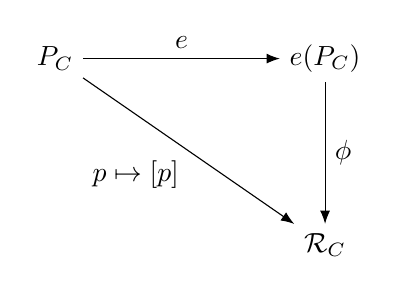
\begin{tikzpicture}[baseline=(current bounding box.center),node distance=18mm and 25mm]
\node (P) {$P_C$};
\node[right=of P] (S) {$e(P_C)$};
\node[below=of S] (R) {$\cR_C$};
\draw[-{Latex}] (P) -- node[above] {$e$} (S);
\draw[-{Latex}] (P) -- node[below left] {$p\mapsto[p]$} (R);
\draw[-{Latex}] (S) -- node[right] {$\phi$} (R);
\end{tikzpicture}
\]
Every transition commutes with $\phi$, and the output factors through
$\cR_C$.  Thus a larger exact state representation may contain caches or
redundancy, but it cannot merge two residual classes.

\subsection{One-way communication interpretation}

At a cut, let Alice know the past $p$ and Bob choose the future $\eta$.  Alice
sends one deterministic message $m(p)$; Bob must output
$O_C(p\cdot\eta)$ for every legal pair.

\begin{proposition}[Deterministic one-way lower bound]
\label{prop:one-way-residual-bound}
Any such exact protocol uses distinct messages for distinct residual classes.
A fixed-width worst-case message therefore has length at least
$\lceil\log_2|\cR_C|\rceil$.
\end{proposition}

\begin{proof}
If $m(p)=m(p')$, Bob behaves identically for every chosen future.  Exactness
then gives $p\equiv_Cp'$.  The counting bound follows.
\end{proof}

This interpretation makes clear why the future class matters: it is Bob's set
of allowed tests.

\subsection{Dense tensor boundary example}

Let the state exposed at a cut be a dense tensor represented as a vector
$T\in\F_q^D$.  If every linear functional
$\ell\in(\F_q^D)^\vee$ is an allowed future observation, then two states are
residually equivalent exactly when they are equal.  Indeed, if $T-T'\ne0$, a
coordinate functional detects a nonzero component.  Hence
\[
  |\cR_C|=q^D,
  \qquad
  \log_2|\cR_C|=D\log_2q.
\]
A direct fixed-width residue encoding uses $D\lceil\log_2q\rceil$ bits.

If only one nonzero functional $\ell$ is allowed, the residual quotient is
instead $\F_q^D/\ker\ell$, which has $q$ classes.  The boundary dimension did
not change; the legal future class did.  Sparse, low-rank, symmetric, or
approximate tensor models change the representation again.

\subsection{Prefix-free variable-length states}

Let $N$ residual classes receive a prefix-free binary code with maximum length
$b$.  Kraft's inequality gives
\[
  1\ge\sum_{i=1}^{N}2^{-\ell_i}
  \ge N2^{-b},
\]
so $b\ge\lceil\log_2N\rceil$.  Without prefix-freeness or another decoding
convention, a raw collection of variable-length strings cannot be counted as a
self-delimiting state code.

Average code length obeys distribution-sensitive entropy bounds, while the
main theorem is a worst-case state-selection statement.  The two should not be
interchanged.

\subsection{Infinite residual spaces}

When $\cR_C$ is infinite, cardinal logarithms do not directly give finite bit
bounds.  One may need:
\begin{itemize}
  \item a topology and covering or packing numbers at scale $\varepsilon$;
  \item a measure and Shannon or mutual information;
  \item a metric loss and rate--distortion function;
  \item an algebraic dimension or rank;
  \item a computable presentation and description-length convention.
\end{itemize}
No one of these is canonical without an application-specific observation and
approximation criterion.

\subsection{Changing future classes}

Let $M_1\subseteq M_2$ be future classes with the same pasts and observation.
Then
\[
  p\equiv_{M_2}p'
  \Longrightarrow
  p\equiv_{M_1}p'.
\]
Thus there is a natural surjection
\[
  P/{\equiv_{M_2}}\longrightarrow P/{\equiv_{M_1}}.
\]
Adding tests refines the residual space; removing tests condenses it.  The
projective passage from left-only futures to arbitrary two-sided futures is a
group-theoretic instance of this general refinement.

\section{Finite network and resource counts}\label{app:network}
% Canonical Paper IV appendix.
The tables below make the finite calibrations reproducible without changing
their interpretation.

\subsection{The finite-field projective tower}

\[
\begin{array}{c@{\qquad}c@{\qquad}c}
|\PP^1(\F_7)|=8,
&|\Biv_{\F_7}^{\mathrm{reg}}|=8\cdot7=56,
&|\PGL_2(\F_7)|=8\cdot7\cdot6=336.
\end{array}
\]
Every bivaluation has six projective-frame lifts.

\subsection{Binary Horner words of length four}

For $k=2$, $n=4$, and Hamming weight two:
\[
\begin{array}{c@{\qquad}c}
\toprule
\text{word }(d_1d_2d_3d_4) & \text{constant in }16x+c\\
\midrule
0011&3\\
0101&5\\
0110&6\\
1001&9\\
1010&10\\
1100&12\\
\bottomrule
\end{array}
\]
All six words have charge $(2,4\log2)$.

For $n=8$, the fixed-weight counts are:
\[
\begin{array}{c|rrrrrrrrr}
m&0&1&2&3&4&5&6&7&8\\
\hline
\binom{8}{m}&1&8&28&56&70&56&28&8&1
\end{array}
\]
The central charge class therefore contains seventy distinct affine operators
in characteristic zero.

\subsection{Free-group ball count}

For the free group $F_r$ with the standard symmetric alphabet of size $2r$,
the sphere of radius $n\ge1$ has
\[
  2r(2r-1)^{n-1}
\]
reduced words.  Hence
\[
  |B(n)|
  =1+2r\frac{(2r-1)^n-1}{2r-2}.
\]
The exponential metric growth coexists with the linear-time stack algorithm
for freely reducing one input word.

\subsection{Finite-field roots and transform networks}

Repeated squaring gives
\[
  3^{128}\equiv256\equiv-1\pmod{257},
  \qquad 3^{256}\equiv1\pmod{257}.
\]
Thus $3$ has order $256$.  The selected roots and network counts are:

\begin{center}
\begin{tabular}{rrrrrr}
\toprule
$N$ & $\zeta_N=3^{256/N}$ & layers & butterflies & $\log_2$ state count & direct bits\\
\midrule
8  &64  &3&12&$8\log_2 257$&72\\
16 &249 &4&32&$16\log_2 257$&144\\
\bottomrule
\end{tabular}
\end{center}

The ``direct bits'' column uses nine bits per field element.  The logarithmic
cardinality is smaller because $257$ is not a power of two.  Twiddle constants
are not included in either dynamic-state column.

\subsection{Matrix-chain calibration}

For dimensions $(100,10,1,2)$:
\[
\begin{array}{c@{\qquad}c@{\qquad}c}
\toprule
plan & \text{scalar multiplications} & \text{principal intermediate entries}\\
\midrule
$(AB)C$ &100\cdot10\cdot1+100\cdot1\cdot2=1200&100\\
$A(BC)$ &10\cdot1\cdot2+100\cdot10\cdot2=2020&20\\
\bottomrule
\end{array}
\]
Peak memory cannot be recovered from the last column without an allocation and
retention policy.

\subsection{Reverse-chain endpoint schedules}

Using Proposition~\ref{prop:reverse-chain-extremes}:
\[
\begin{array}{c@{\qquad}c@{\qquad}c@{\qquad}c}
\toprule
$N$ & \text{store-all work} & \text{naive recompute work} & \text{extra prefix work}\\
\midrule
8  &16&44&28\\
16 &32&152&120\\
\bottomrule
\end{array}
\]
The work convention charges one unit per forward local evaluation and one per
reverse local step.  It excludes instruction, communication, and variable-size
state costs.

\section{Claim ledger and cost-model checklist}\label{app:ledger}
% Canonical Paper IV appendix.
This ledger records the status and boundary of the principal Paper~IV claims.
``Proved'' means that a proof appears in the active manuscript under the stated
hypotheses.  ``Framework'' denotes a definition or proposed architecture, not
a theorem of machine independence.

\subsection{Claim ledger}

\begingroup\setlength{\tabcolsep}{4pt}\begin{longtable}{L{0.10\textwidth}L{0.36\textwidth}L{0.13\textwidth}L{0.24\textwidth}}
\toprule
ID & Claim & Status & Boundary\\
\midrule
\endfirsthead
\toprule
ID & Claim & Status & Boundary\\
\midrule
\endhead
PIV-H0 & Histories, operators, bivaluations, projective points, and endpoints form distinct equality levels. & Proved by definitions and examples & Ordinary-domain labels remain separate from projective continuation.\\
PIV-P1 & Regular bivaluations are rank-one idempotents. & Proved, Theorem~\ref{thm:bivaluation-projector} & Requires transverse ordered lines.\\
PIV-P2 & $G/H\cong\Biv_K^{\mathrm{reg}}$ and $G\to G/H$ is a frame torsor. & Proved & No canonical connection over an arbitrary field.\\
PIV-P3 & Finite-field quotient and fiber counts are exact. & Proved & Algebraic count, not dynamical attraction.\\
PIV-C1 & A left-equivariant quotient with injective identity observation is the exact residual. & Proved & Depends on descended action and observation.\\
PIV-C2 & One right update descends iff $k^{-1}Hk\subseteq H$. & Proved & Inclusion need not be equality for infinite $H$.\\
PIV-C3 & Reversible right continuation acts iff it lies in $N_G(H)$. & Proved & Applies to right action on the selected right-coset quotient.\\
PIV-R1 & Contextual residual equivalence is a right congruence. & Proved & Requires totalized partial action.\\
PIV-R2 & The residual quotient is the canonical minimal exact deterministic state. & Proved & Exact deterministic online model only.\\
PIV-R3 & Finite residuals lower-bound fixed-width or prefix-free maximum state length. & Proved & Not transition-table or average-code size.\\
PIV-R4 & Summed residual bounds give fixed-register capacity--time. & Proved & Actual memory--time only under the declared snapshot charging rule.\\
PIV-S0 & Ported AES carriers separate geometric ends, computational holes, and input/output ports. & Structural proposal & Port anchoring does not realize gates as AES motions.\\
PIV-S1 & Typed finite substitution preserves sources and instantiated occurrences. & Proved with stated hypotheses & Complete one-use bindings; explicit copy/discard; global DAG.\\
PIV-S2 & Substitution commutes with strict partial evaluation on the exact composite domain. & Proved, Theorem~\ref{thm:ported-substitution-evaluation} & Pure deterministic primitives; discarded producers still execute.\\
PIV-S3 & Composition is associative for partial maps and up to explicit isomorphism for operation networks. & Proved & Domains agree; literal receipts remain distinct; boundary orders must match.\\
PIV-S4 & Compatible collars and computational interfaces descend together. & Proved with stated hypotheses & Smooth Hausdorff carrier, equal signed parameters, compatible full seam data and global DAG.\\
PIV-S5 & Feature observations factor iff feature fibers refine contextual equivalence. & Proved, Theorem~\ref{thm:feature-observation-descent} & Declared futures and invalid outcome; no effectiveness claim.\\
PIV-S6 & Online feature updates exist iff the feature kernel is a right congruence. & Proved, Proposition~\ref{prop:feature-online-update} & An exact machine also needs current-output factorization.\\
PIV-S7 & The four-input scalar experiment outputs $(9,15,5/2)$. & Exact finite example & Attached network; not Adva's native output roles or an AES gate-motion realization.\\
PIV-O1 & Ever-computed node sets do not determine workspace with erasure or recomputation. & Proved & Requires a positive-size optional live value.\\
PIV-G1 & Maximum fiber size is at least raw words divided by image size. & Proved & Cardinality only.\\
PIV-G2 & Conditional lost information obeys Equation~\eqref{eq:conditional-information-loss}. & Proved & Uniform word distribution in the displayed form.\\
PIV-W1 & Additive potential labels telescope. & Proved & Single-valued additive potential.\\
PIV-W2 & Pure-gauge group labels telescope. & Proved & Does not exclude non-flat connections.\\
PIV-H1 & Fixed digit histograms give multinomially many distinct Horner operators with one ACS charge. & Proved & Characteristic zero; fixed radix and length.\\
PIV-B1 & Equality OBDD width is exponential in block order and constant in interleaved order. & Proved & Fixed OBDD model and variable order.\\
PIV-N1 & $\mathsf B_\omega=\mathsf B_1D_\omega$ and all twiddles share one right $H$-coset. & Proved & Local $2\times2$ statement, $\operatorname{char}K\ne2$.\\
PIV-N2 & Radix-two layer, cell, and invertible layer-state counts are exact. & Proved & Fixed breadth-first topology and full input range.\\
PIV-T1 & Matrix chains and reverse schedules realize exact work--space tradeoffs. & Proved in stated elementary models & Not a universal optimality theorem.\\
PIV-F1 & Pareto resource geometry organizes uniform realizations. & Framework & Model, units, precision, and simulations must be fixed.\\
PIV-F2 & Faithful multi-wire AES motion realizations and actual opposite-edge features. & Open problems & The finite ported-network interface is established; geometric gate realization and native feature witnesses are not.\\
PIV-F3 & Projective rewrite holonomy extends affine torsion: the four-step loop carries the cross-ratio holonomy $\Lambda(\square)$ with a linear witness. & Proved, Theorem~\ref{thm:projective-torsion-solution} & Incidence-coupled rank-one transport; reduces to the affine cocycle on the Borel sector. Normalisation of the density against the reductive-connection curvature remains open and is recorded in Section~\ref{sec:boundaries}.\\
PIV-X1 & Noncommutativity, curvature, group growth, and raw fibers imply hardness. & Excluded & No such implication appears in the active claims.\\
\bottomrule
\end{longtable}
\endgroup

\subsection{Cost-model checklist}

Before any complexity comparison is promoted to a theorem, the manuscript or
experiment must state:

\begin{enumerate}
  \item the input family and size parameter;
  \item the semantic task and exact, randomized, or approximate success rule;
  \item the history, circuit, network, proof, or machine language;
  \item uniformity and preprocessing;
  \item ordinary-domain and type-error conventions;
  \item value, instruction, constant, and output encodings;
  \item atomic actions and their weights;
  \item processor, memory, and communication topology;
  \item live-state legality, erasure, and recomputation rules;
  \item whether input, output, tables, code, and constants count toward space;
  \item precision, conditioning, and numerical stability when applicable;
  \item the continuation class and observation defining residuals;
  \item the exact comparison or simulation relating the models.
\end{enumerate}

A missing item does not make a calculation useless; it limits which resource
claim the calculation can support.

\subsection{Case-study matrix}

\begin{center}
\begin{tabular}{L{0.17\textwidth}L{0.23\textwidth}L{0.23\textwidth}L{0.25\textwidth}}
\toprule
Example & Semantic quotient & Operational object & Main lesson\\
\midrule
ported AES & program substitution $\to$ strict partial evaluation & explicit-copy DAG and call receipts & attached program semantics do not realize AES gate motions\\
Horner & word $\to$ operator $\to$ ACS charge & streaming accumulator & large charge class can be easy to evaluate\\
OBDD equality & prefixes $\to$ residual Boolean functions & decision-diagram nodes & cut order can change width exponentially\\
NTT & dense transform $\to$ factored network; local $G/H$ coset & wire layers and twiddle storage & static labels and dynamic state differ\\
matrix chain & parenthesizations of one product & intermediate matrices & equal semantics have incomparable resource vectors\\
reverse chain & one derivative map & checkpoints and recomputation trace & completed sets do not encode live space\\
rewrite loop & semantic fiber & edge actions and $2$-cells & exact potentials are not holonomy\\
\bottomrule
\end{tabular}
\end{center}

\subsection{Release status}

This manuscript is a mathematical-review integration.  It promotes the proved
finite and algebraic results listed above, while keeping machine-independent
complexity, faithful multi-wire AES motion realizations, actual opposite-edge
feature witnesses, projective holonomy, and approximate residuals open.
It does not alter the release or DOI status of Papers~I--III.  Public release,
author metadata, and DOI assignment remain subject to explicit author approval.


\bibliographystyle{plain}
\bibliography{../bibliography/aeg-paper}
\end{document}
